\chapter{Betriebsdokumentation}
Die Betriebsdokumentation beschreibt die Schritte, die ausgeführt werden müssen, um die einzelnen Komponenten in der Produktivumgebung zu deployen und die einzelnen Komponenten zu warten. Darüber hinaus wird für bestimmte Komponenten ein Nutzerhandbuch angeboten. Ebenso wird auf bestimmte Einschränkungen und bekannte Fehler eingegangen.

\section{Deployment Produktiv-System}
In diesem Abschnitt wird für die einzelnen Komponenten des Systems das Deployment auf die Produktiv-Systeme betrieben. 
Für diese Anleitungen ist informationstechnisches Wissen vorteilhaft. 


\subsection{IoT-Plattform}
In diesem Abschnitt wird das Deployment der IoT-Plattform auf dem Produktiv-System beschrieben. 
Das Deployment auf dem Produktiv-System ähnelt dem Deployment auf dem Development-System sehr stark, denn auch hier wird dafür docker-compose verwendet. 
Im Folgenden werden die Schritte genannt, die erforderlich sind, um die IoT-Plattform produktiv zu deployen. \newline
\begin{enumerate}
	\item Zuerst muss sich der Entwickler auf die VM einloggen
	\item Danach müssen die \textit{env.} Datein angelegt oder gegebenenfalls angepasst werden. Die \textit{env.} Dateien wurden bereits im Dokument 2 in Abschnitt 3.3.4.1 erläutert. Insbesondere muss hier auf die Anpassung der Pfade, zum Beispiel die der Datenbank, geachtet werden. \newline
	Wenn beispielsweise ein neuer Microservice deployed werden soll muss eine neue \textit{env.} Datei angelegt werden. Unter \textit{home/pgrio/microservices/} muss nun ein neuer Ordner BeispielMicroservice angelegt werden, der die \textit{env.} Datei enthält \newline
	Die \textit{env.} Datei muss den folgenden Inhalt haben: \newline
	\begin{lstlisting}[language=json,firstnumber=1,basicstyle=\footnotesize]
	DB_URL = ProduktivDatenbankURL
	API_GATEWAY_URL = ProduktivAPIGatewayURL
	SERVICE_USERNAME = BeispielMicroservice
	SERVICE_PASSWORD = BeispielMicroservicePassword
	RENEW_INTERVALL = 5
	SERVICE_PORT = 3102
	SERVICE_HOST = beispielmicroservice
	\end{lstlisting}
	\begin{itemize}
		\item DB\_URL: URL der Datenbank, die auf dem Produktiv-System läuft
		\item API\_GATEWAY\_URL: URL des API Gateways, das auf dem Produktiv-System läuft
		\item SERVICE\_USERNAME: Der Benutzername des Microservices, der auch in der Datenbank hinterlegt ist
		\item SERVICE\_PASSWORD: Das Passwort des Microservices, das auch in der Datenbank hinterlegt ist
		\item SERVICE\_PORT: Der Port des Microservices, auf dem der Microservice erreichbar ist. Dieser ist nur dür das API Gateway offen und nicht außerhalb des Docker Netzwerkes
		\item RENEW\_INTERVAL Das Zeitintervall, in dem der Microservice ein neues Token anfragt
		\item SERVICE\_HOST: Entspricht dem Namen des Microservices in der yaml Datei und ist notwendig, damit das API Gateway die Anfragen, an der richtigen Microservice weiterleiten kann
		\end{itemize}
	\item Nachdem die \textit{env.} Dateien erstellt wurden muss die yaml Datei angepasst werden. Für das zuvor genannte Beispiel, einen neuen Microservice zu deployen, ist die Anpassung der yaml Datei ab Zeile 85 notwendig. Folgend ist die aktuelle yaml Datei der Produktionsumgebung gezeigt: \newline
	\begin{lstlisting}[language=json,basicstyle=\footnotesize]
	version: '3.5'
	services:
	mqttbroker:
	image: pgrio/iot-mqtt-broker-hive:stable
	volumes:
	- /home/pgrio/iot-platform/mqtt/config.properties:/opt/hivemq/config.properties
	ports:
	- "127.0.0.1:1883:1883"
	restart: always
	depends_on:
	- identityservice
	identityservice:
	image: pgrio/iot-identity-service:stable
	volumes:
	- /home/pgrio/iot-platform/identityservice/production.env:/usr/src/app/production.env
	environment:
	- NODE_ENV=production
	expose:
	- "9090"
	restart: always
	depends_on:
	- collection_creater
	api_gateway:
	image: pgrio/iot-api-gateway:stable
	volumes:
	- /home/pgrio/iot-platform/apigateway/production.env:/usr/src/app/production.env
	environment:
	- NODE_ENV=production
	ports:
	- "127.0.0.1:8080:8080"
	restart: always
	depends_on:
	- identityservice
	iot-data-collector:
	image: pgrio/iot-data-collector:stable
	volumes:
	- /home/pgrio/iot-platform/datacollector/config.env:/usr/src/app/config.env
	environment:
	- NODE_ENV=production
	restart: always
	depends_on:
	- collection_creater
	collection_creater:
	image: pgrio/iot-collection-creater:stable
	volumes:
	- /home/pgrio/iot-platform/collectioncreater/config.env:/usr/src/app/config.env
	environment:
	- NODE_ENV=production
	pm25microservice:
	image: pgrio/iot-microservice-pm25:stable
	expose:
	- "3000"
	volumes:
	- /home/pgrio/iot-platform/microservices/pm25/production.env:/usr/src/app/production.env
	environment:
	- NODE_ENV=production
	restart: always
	tempmicroservice:
	image: pgrio/iot-microservice-temp:stable
	expose:
	- "3004"
	volumes:
	- /home/pgrio/iot-platform/microservices/temp/production.env:/usr/src/app/production.env
	environment:
	- NODE_ENV=production
	restart: always
	svmicroservice:
	image: pgrio/iot-microservice-sv:stable
	expose:
	- "3002"
	volumes:
	- /home/pgrio/iot-platform/microservices/sv/production.env:/usr/src/app/production.env
	environment:
	- NODE_ENV=production
	restart: always
	uismicroservice:
	image: pgrio/iot-microservice-uis:stable
	expose:
	- "3001"
	volumes:
	- /home/pgrio/iot-platform/microservices/uis/production.env:/usr/src/app/production.env
	environment:
	- NODE_ENV=production
	restart: always
	beispielmicroservice:
	image: pgrio/iot-microservice-beispiel:stable
	expose:
	- "3102"
	volumes:
	- /home/pgrio/iot-platform/microservices/BeispielMicorservice/production.env:/usr/src/app/production.env
	environment:
	- NODE_ENV=production
	restart: always
	\end{lstlisting}
	\begin{itemize}
		\item image: Der Name des Image, wie er auf Docker-Hub veröffentlicht wurde. Außerdem wird die Versionierung angegeben
		\item expose: Der Port unter dem der Service intern erreichbar ist
		\item volumes: Der Pfad, unter dem die \textit{env.} Datei des Service zu finden ist
		\item environment: Setzt die Umgebungsvariable auf eine Umgebungsdatei. Sobald der Container gestartet wird, hat die definierte Umgebungsvariable Vorrang
		\item restart: In diesem Fall werden die Container immer neu gestartet
	\end{itemize}
	\item Der Unterschied zum Deployment auf der Development Umgebung ist die Versionierung der Images. Für die Produktiv Umgebung wird die Version \textit{stable} verwendet, siehe dazu unter \textit{image} in der yaml Datei
	\item Sobald der Master eines Repositoriums der IoT-Plattform aktualisiert wurde veröffentlicht der Jenkins ein neues Image mit der Versionierung \textit{stable}
	\item Für das Beispiel, das Deployment eines neuen Microservices, ist es notwendig das aktuelle Image von Docker Hub zu beziehen. Dieser Schritt ist ebenfalls notwendig, wenn der Jenkins ein anderes Image der IoT-Plattform aktualisiert hat. Mit dem folgenden Befehl wird das aktuellste Image von Docker Hub bezogen: \newline
	\console{docker pull pgrio/iot-microservice-beispielmicroservice:stable} (\textit{imagename:stable})
	Insbesondere muss hier die Versionierung des Image angegeben werden. Auf dem Deployment-System ist dies nicht notwendig, da die Standardversionierung \textit{latest} ist
	\item Mit dem Befehl \console{docker-compose up} kann nun die IoT-Plattform auf dem Produktiv-System gestartet werden. \newline
	Falls bereits Container aktiv sind, muss die IoT-Plattform nicht komplett heruntergefahren werden, wenn ein neuer Service deployed wurde oder lediglich ein neues Image eines Containers verfügbar ist. Mit dem zuvor genannten Befehl werden die Container neu gestartet, die ein neues Image besitzen
\end{enumerate}

\subsection{Routing}
In diesem Abschnitt wird das Deployment des Routing Dienstes auf die Umgebung produktiv beschrieben. 
Für das Deployment muss eine jar-Datei von dem Projekt erstellt werden. 
Dieser Vorgang wird in der Entwicklerdokumentation beschrieben. 
Diese jar-Datei muss auf die VM mit der Adresse \textit{pg-rio-routing.informatik.uni-oldenburg.de} in dem Ordner \textit{/home/pg-rio} installiert werden. 
Dann muss der Befehl \textit{java -jar routing-backend.jar} in diesem Ordner ausgeführt werden. 
Somit ist die Applikation gestartet und kann über die Adresse der VM erreicht werden.

\subsection{Sensorknoten}
Um den Betrieb und die Installation der Sensorknoten-Firmware zu ermöglichen, muss die aktuelle Version auf dem Update-Server bereitgestellt werden.
Diese steht dann im Installationstool zum Flashen auf dem Sensorknoten zur Verfügung. Die Installation und Konfiguration ist in \Fref{sec:nutzerhandbuch:sk} erklärt. Zusätzlich aktualisieren sich Sensorknoten im laufenden Betrieb auf eine aktuellere Version, falls sie auf dem Server bereitsteht.

Firmware"=Updates werden per HTTPS vom Server \url{https://pg-rio-sensors-update.informatik.uni-oldenburg.de} bezogen.
Dieser muss dazu im Webroot eine JSON"=Datei mit dem Namen \filename{availableUpdates.json} und folgendem Aufbau bereitstellen:
\begin{lstlisting}[language=json]
{
  "updates": [
    {
      "_v": "1",
      "path": "/realtivePathTo.bin",
      "version": "version",
      "crc32": "crc32inLowerLetters",
      "description": "Description"
    },
    {
      "_v": "1",
      "path": "/files/empty.bin",
      "version": "0.0.190911000000",
      "crc32": "deadbeef",
      "description": "Example-File"
    }
  ]
}
\end{lstlisting}

Die Firmware"=Datei wird dann relativ zur \filename{availableUpdates.json} abgelegt, hier im Beispiel im Verzeichnis \dirname{files}.
Da der Puffer für die \filename{availableUpdates.json}"=Datei auf dem Sensorknoten begrenzt ist, sollten nicht mehr als fünf Versionen in der Datei zur Verfügung stehen.
Die Auswertung der \filename{availableUpdates.json} geschieht dann "von oben nach unten", wobei die erste Firmware mit neuerer Version ausgewählt und heruntergeladen wird.
Dieses Vorgehen ermöglicht eine gezielte Sequenzialisierung der Updates, sofern einmal eine Interims"=Firmware benötigt werden sollte. 
 

\section{Wartung}
Im Folgenden werden die Möglichkeiten beschrieben, um die einzelnen Komponenten des Systems zu warten. 
Da die einzelnen Komponenten unterschiedlich komplex sind, ist der Umfang der Wartungsmöglichkeit sehr unterschiedlich.

\subsection{IoT-Plattform}
In diesem Abschnitt wird erläutert, wie die IoT-Plattform gewartet werden kann. 
Insbesondere wird im folgenden auf die Fehlerbehebung eingegangen. 
Falls die IoT-Plattform oder einer der Services der IoT-Plattform nicht erreichbar ist, wird dies an zwei Stellen deutlich. Entweder können externe Dienste die IoT-Plattform nicht mehr erreichen oder die Sensorknoten können keine Daten mehr an den MQTT-Broker senden. Für diese beiden groben Fehlerquellen werden im Folgenden Problemerkennungs - und Lösungsmaßnahmen aufgezeigt. \newline
Falls die IoT-Plattform für die externen Dienste nicht mehr erreichbar ist kann dies entweder an dem API-Gateway, dem Identity-Service oder an einem der Microservices liegen. 
Für die Fehlererkennung ist es empfehlenswert die Logs des Containers auf der VM anzuschauen. Dafür sind folgende Schritte notwendig:
\begin{enumerate}
	\item Mit dem Befehl \console{docker ps} werden alle aktiven Container angezeigt. Um sich die Logs eines Containers anschauen zu können muss die ID des Containers bekannt sein
	\item Bei dem Aufruf wird nicht nur die ID aller aktiven Container angezeigt, sondern auch deren Laufzeit. Falls sich ein Container immer wieder neu startet wird das hier deutlich, da dieser dann erst seit ein paar Sekunden wieder aktiv ist. Falls dem so ist, sollten sich die Logs dieses Containers zuerst angeschaut werden. Dies tritt beispielsweise bei den Microservices auf, wenn diese sich nicht an dem API-Gateway authentifzieren können. Gründe hierfür können sein: fehlende Parameter in der env Datei oder falsche Zugangsdaten des Microservices in der Datenbank hinterlegt.
	\item Mit dem Befehl \console{docker logs \textit{Container ID}} werden die Logs des Containers angezeigt. In den meisten Fällen zeigen die Logs das Problem an
	\item Bug lösen und danach mit dem jeweiligen Branch, entweder Develop oder Master, zusammenführen
	\item Nachdem Jenkins das Image auf Docker Hub veröffentlicht hat kann mit \console{docker pull \textit{Image Name}} das aktuellste Image von Docker Hub bezogen werden
	\item Mit \console{docker-compose up} die IoT-Plattform starten
\end{enumerate}
Folgend werden Fehler augfelistet, die häufig auftreten:
\begin{enumerate}
	\item Imports innerhalb des Codes. Sobald ein fixer Pfad angegeben wird, findet das Projekt die Imports nicht und wirft deshalb Fehler
	\item Außerdem starten sich die Projekte nicht neu, wenn eine Datenbankverbindung auftritt. Das hat zur Folge, dass sich die Projekte danach nicht mehr mit der Datenbank verbinden und somit Fehler werfen. Dieses Problem ist ein bekannter Bug und wird ebenfalls in  \Fref{sec:bugsundeinschraenkungen} aufgeführt
	\item Microservice kann sich nicht an dem API-Gateway authentifizieren, wie zuvor bereits erwähnt
\end{enumerate}
Falls das Problem mit Hilfe der Logs nicht bekannt wird, ist es hilfreich den betreffenden Container neu zu starten. Um zu filtern, welcher Container gestoppt werden sollte, ist es hilfreich die nicht funktionierenden Abfragen zu definieren. 
\begin{itemize}
	\item Falls sich der externe Dienst nicht authentifizieren kann, also kein Token abfragen kann, sollte der API-Gateway-Container neu gestartet werden
	\item  Falls das Problem danach weiterhin besteht, sollte zusätzlich der Identity-Service-Container neu gestartet werden
	\item  Wenn sich ein externer Dienst jedoch authentifizieren kann und lediglich keine Antwort eines Microservices bekommt, sollte der jeweilige Microservice neu gestartet werden
\end{itemize}
Sobald herausgefunden wurde, welcher Container gestoppt und neu gestartet werden sollte, müssen folgende Schritte ausgeführt werden: 
\begin{enumerate}
	\item \console{docker stop \textit{Container ID}}
	\item \console{docker-compose up}
	\item \console{docker ps}, um zu kontrollieren, ob der Container erfolgreich neu gestartet wurde
\end{enumerate}

Eine weitere Schnittstelle zur IoT-Plattform bietet der MQTT-Broker. 
Falls an dieser Schnittstelle Fehler auftreten wird dies deutlich, wenn Sensorknoten keine Daten mehr an die IoT-Plattform senden. Gründe dafür können zum einen der MQTT-Broker sein oder zum anderen der Data-Collector. Für die Fehlerbehebung an dieser Schnittstelle sind folgende Schritte empfehlenswert:
\begin{enumerate}
	\item Zuerst sollte geprüft werden, ob Daten der Sensorknoten an dem MQTT-Broker ankommen
	\item Falls dies nicht der Fall ist, sollten sich die Logs des MQTT-Broker-Containers angeschaut werden
	\item Falls die Daten ankommen, aber nicht in der Datenbank gespeichert werden sollten sich die Logs des Data-Collector-Containers angeschaut werden
\end{enumerate}
Das Vorgehen zum Anzeigen der Logs wurde zuvor bereits erläutert. Wie auch bei der anderen Schnittstelle, sollte erst danach der Container gestoppt und neu gestartet werden, falls das Problem weiterhin besteht. 


\subsection{Routing}
In diesem Abschnitt wird beschrieben, wie der Routing-Dienst gewartet wird. 
Diese Tätigkeit ist bei dieser Komponente nicht sehr aufwändig, da der Dienst von der Architektur her einfacher konstruiert ist. 
Um mögliche Fehler schneller analysieren zu können, besitzt der Dienst umfangreiche Debug-Ausgaben. Dazu können in der Terminal-Session, in welcher der Dienst gestartet wurde, diese Ausgaben angeschaut und bei ungewollten Verhalten entsprechend reagiert werden.

\section{Nutzerhandbuch Navigations"=App}
Die Projektgruppe RIO bietet eine Anwendung für Handynutzer, mit deren Hilfe Sie in Oldenburg anhand Umwelt Parametern navigieren können.\\
Die folgenden Schritte zeigen Ihnen, wie Sie die App einrichten und benutzen können.
 
\subsection{Anwendung starten}

\begin{itemize}
	\item Laden Sie die RIO Navigation Anwendung herunter und installieren Sie diese.
  \item Öffnen Sie auf Ihrem Handy die RIO Navigation Anwendung.
  \item Tippen Sie oben links auf die Menüschaltfläche, um die Routeninformationen zu öffnen.
\end{itemize}
Wie gezeigt in \Fig{app:starten}.
\begin{figure}[h!]
\centerline{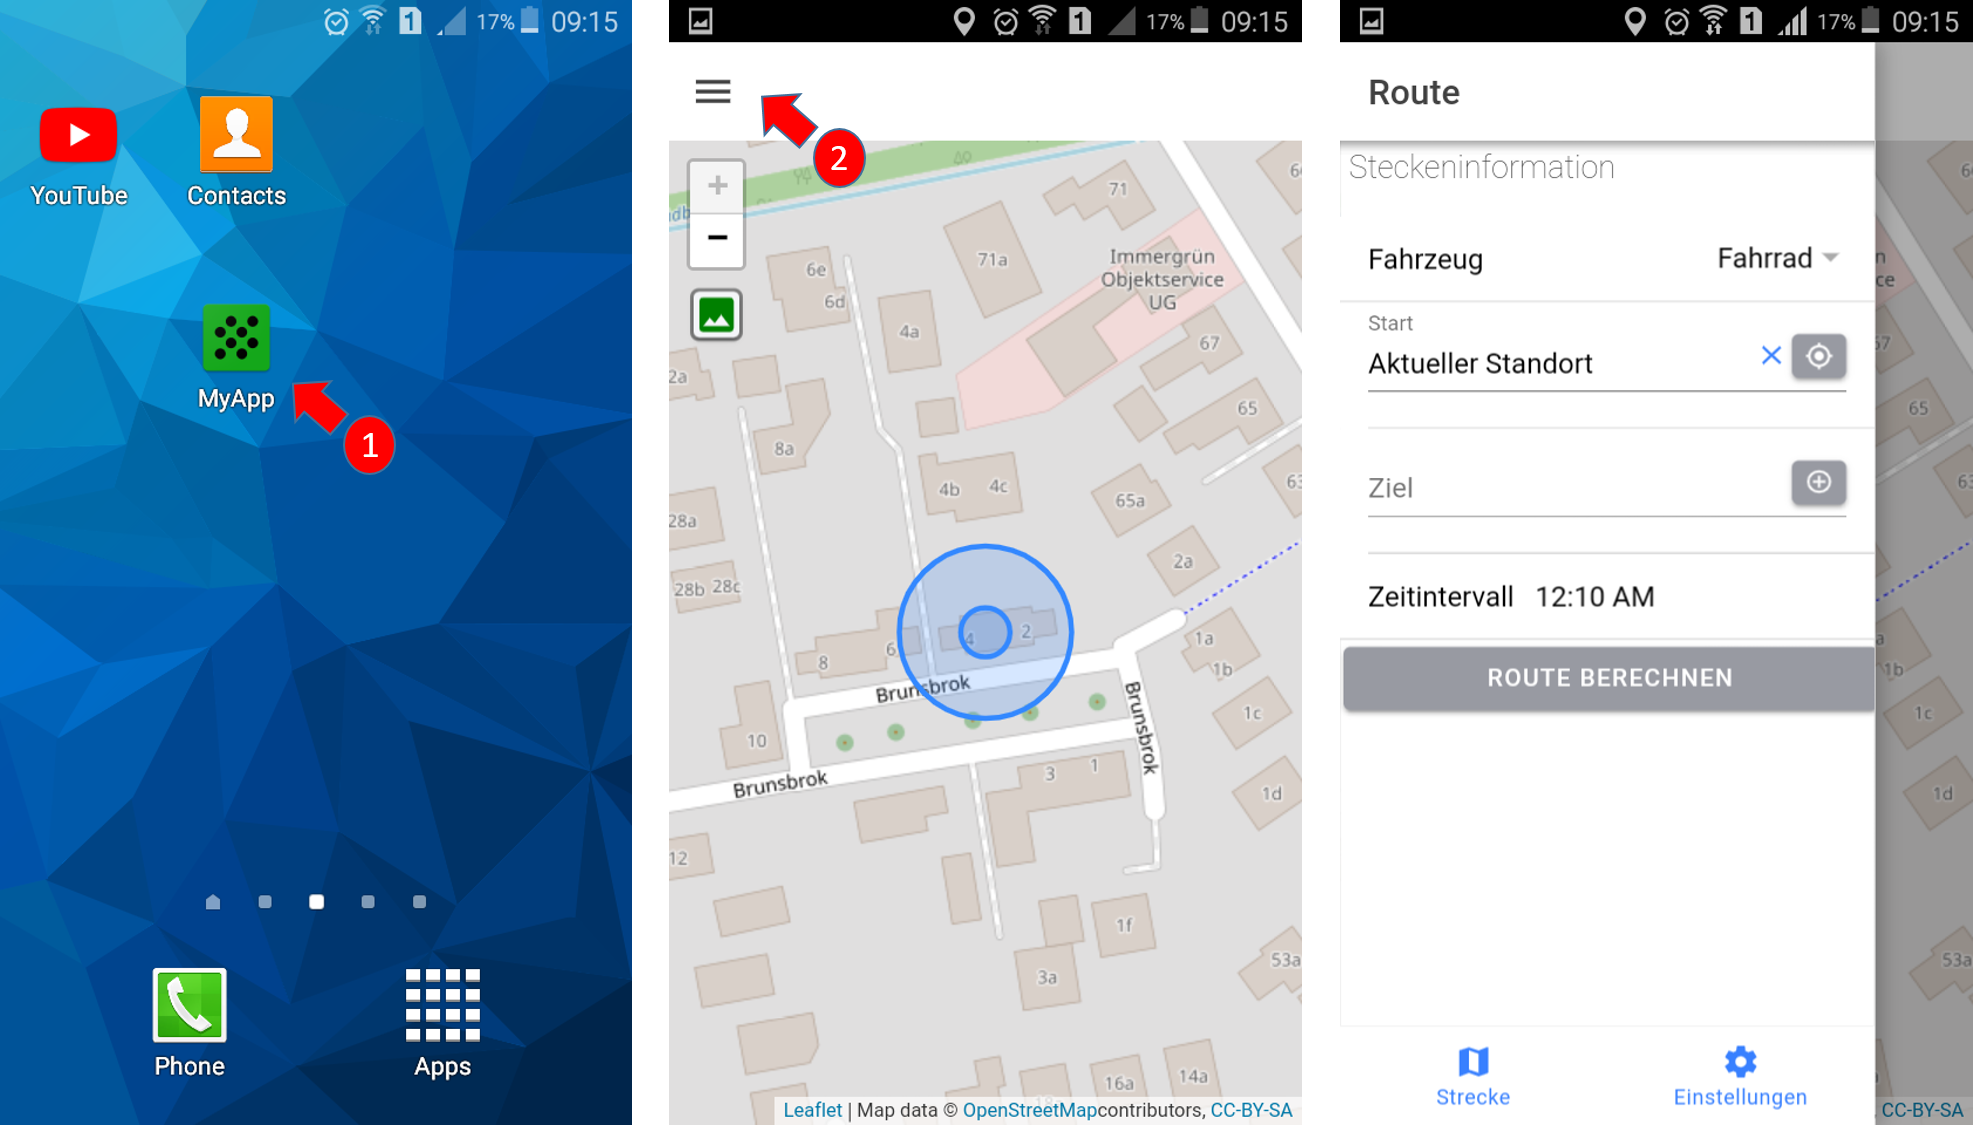
\includegraphics[height=8 cm]{./ressourcen/nutzerhandbuch/start_up.png}}
\caption{RIO Navigation Anwendung starten.}
\label{fig:app:starten}
\end{figure}

\newpage
\subsection{Route berechnen und Routen anzeigen}
\paragraph{Startpunkt:}
Suchen Sie nach Ihrem Start oder tippen Sie auf der Karte auf den gewünschten Startpunkt.\\
Wie gezeigt in \Fig{app:Startpunkt}.
\begin{figure}[h!]
\centerline{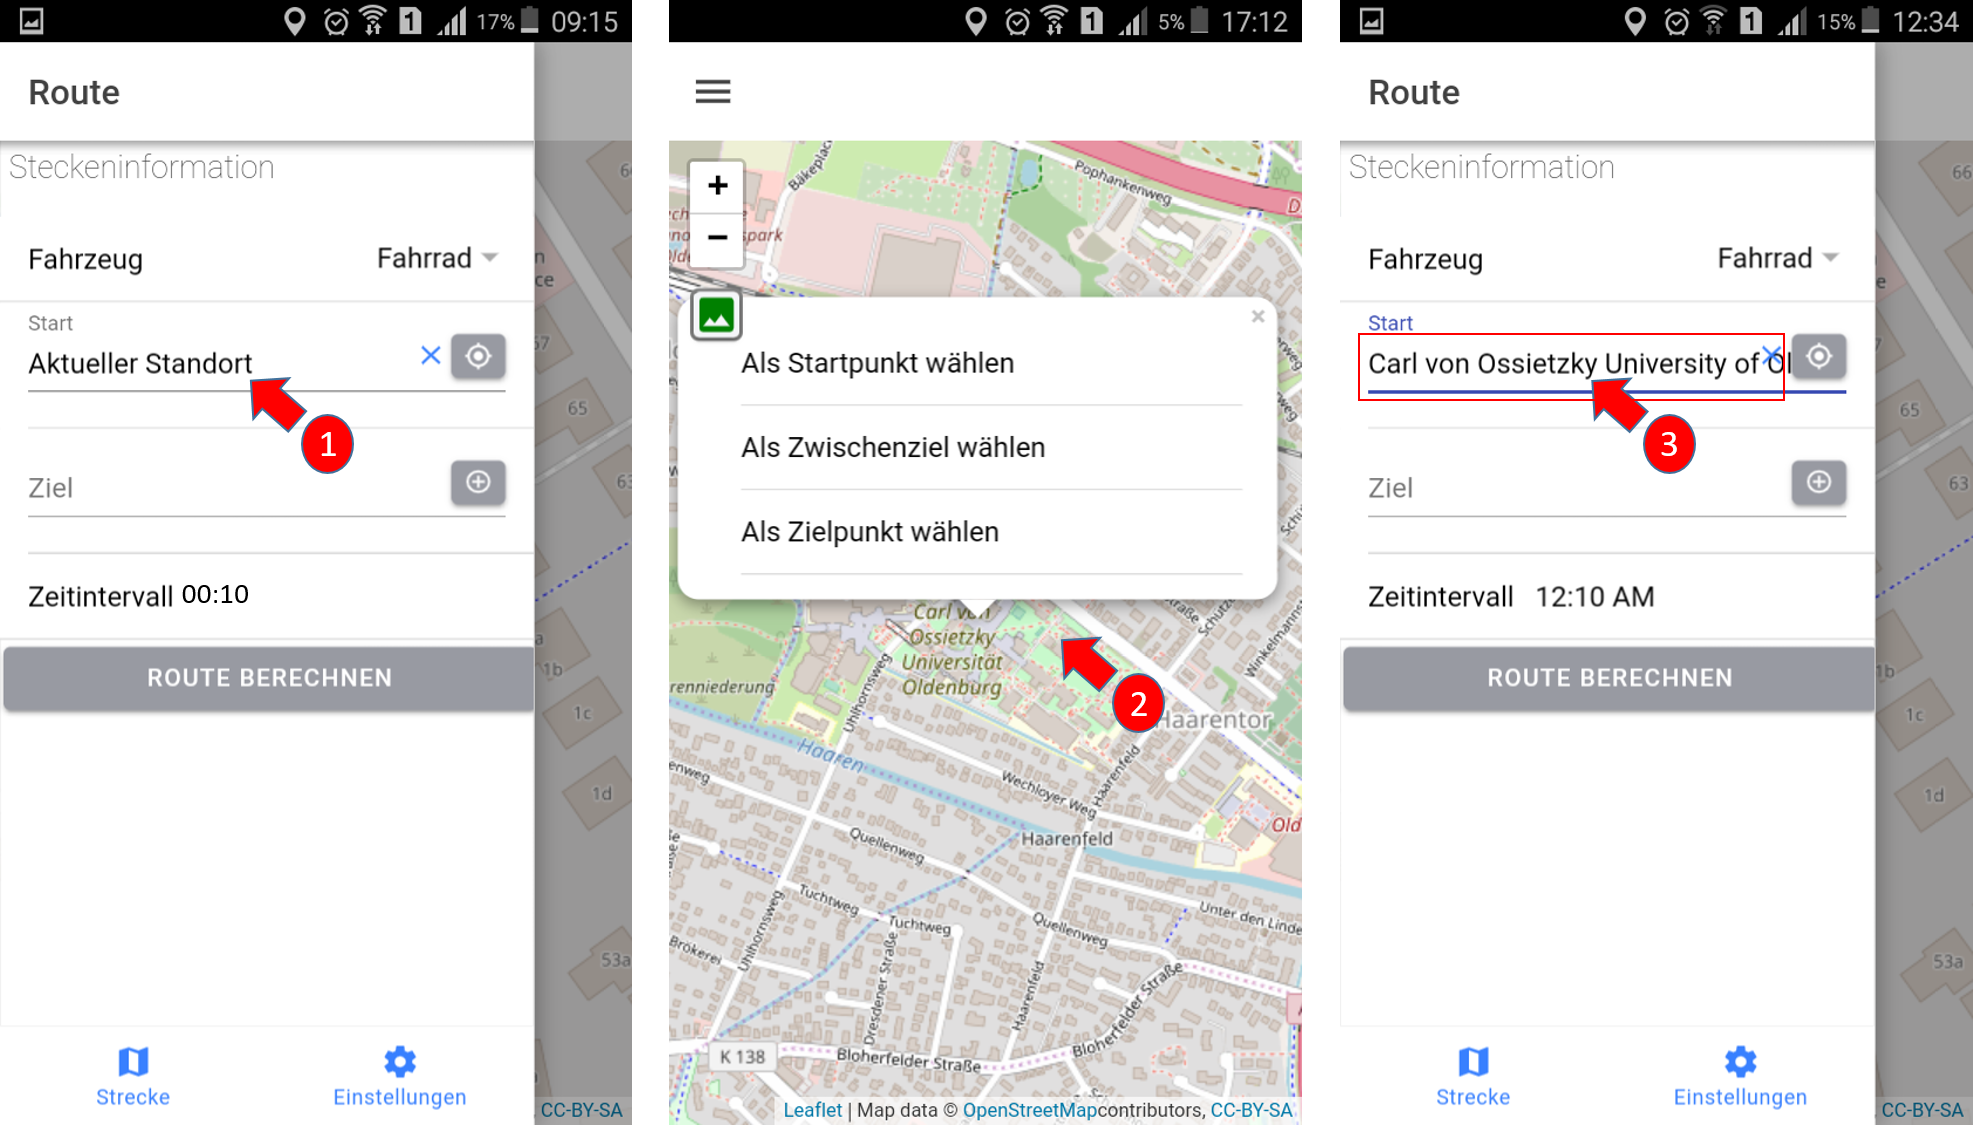
\includegraphics[height=8 cm]{./ressourcen/nutzerhandbuch/start.png}}
\caption{Startpunkt wählen}
\label{fig:app:Startpunkt}
\end{figure} 

\newpage

\paragraph{Zwischenziele:}
\begin{itemize}
  \item Um ein Zwischenziel hinzuzufügen, klicken Sie auf das Plus-Symbol rechts neben dem Zieleingabefeld.
  \item Suchen Sie nach Ihrem Zwischenziel oder tippen Sie auf der Karte auf das gewünschte Zwischenziel.
\end{itemize}
Wie gezeigt in \Fig{app:Zwischenziel}.
\begin{figure}[h!]
\centerline{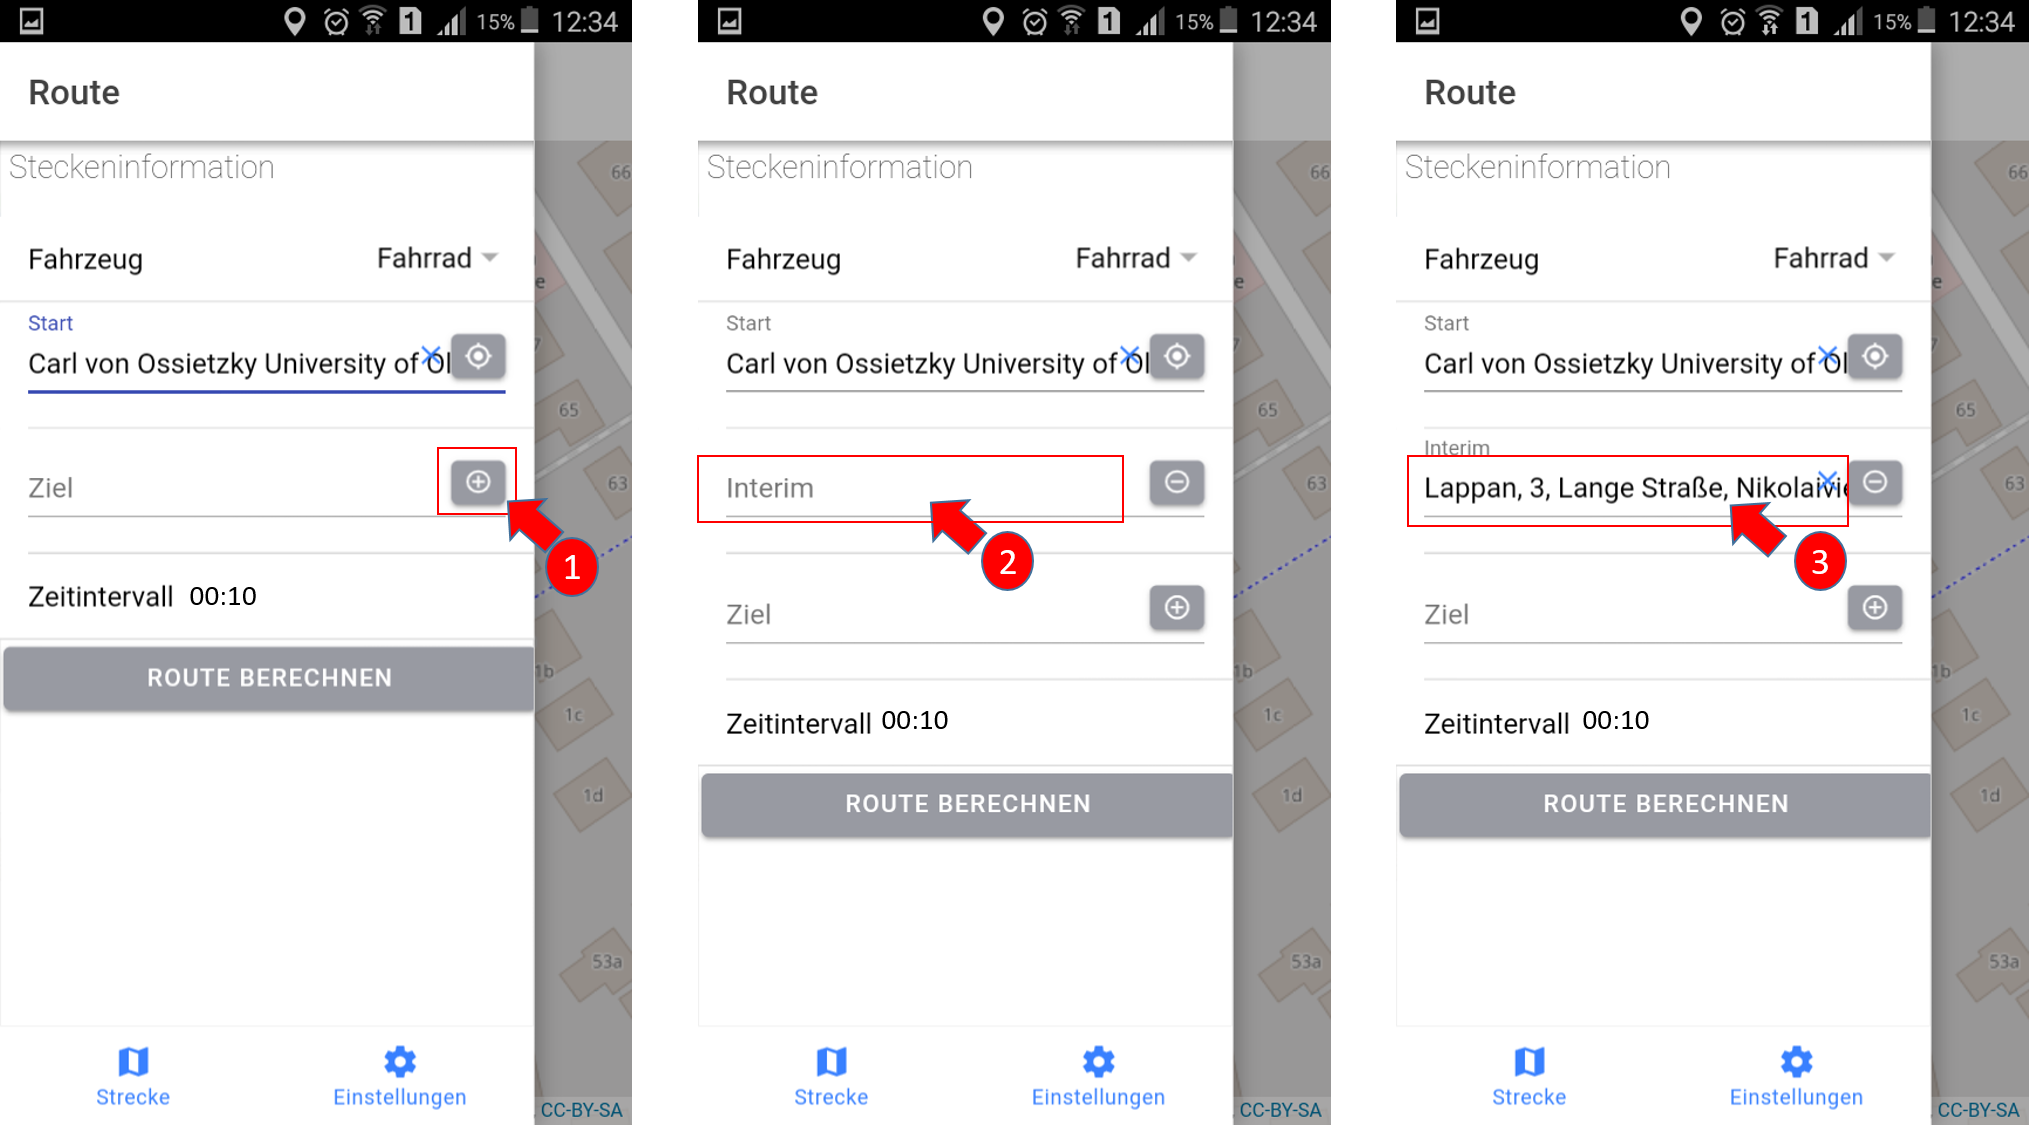
\includegraphics[height=8 cm]{./ressourcen/nutzerhandbuch/intrim.png}}
\caption{Zwischenziel hinzufügen}
\label{fig:app:Zwischenziel}
\end{figure} 

\newpage

\paragraph{Zielpunkt:}
Suchen Sie nach Ihrem Ziel oder tippen Sie auf der Karte auf das gewünschte Ziel.\\
Wie gezeigt in \Fig{app:Zielpunkt}.
\begin{figure}[h!]
\centerline{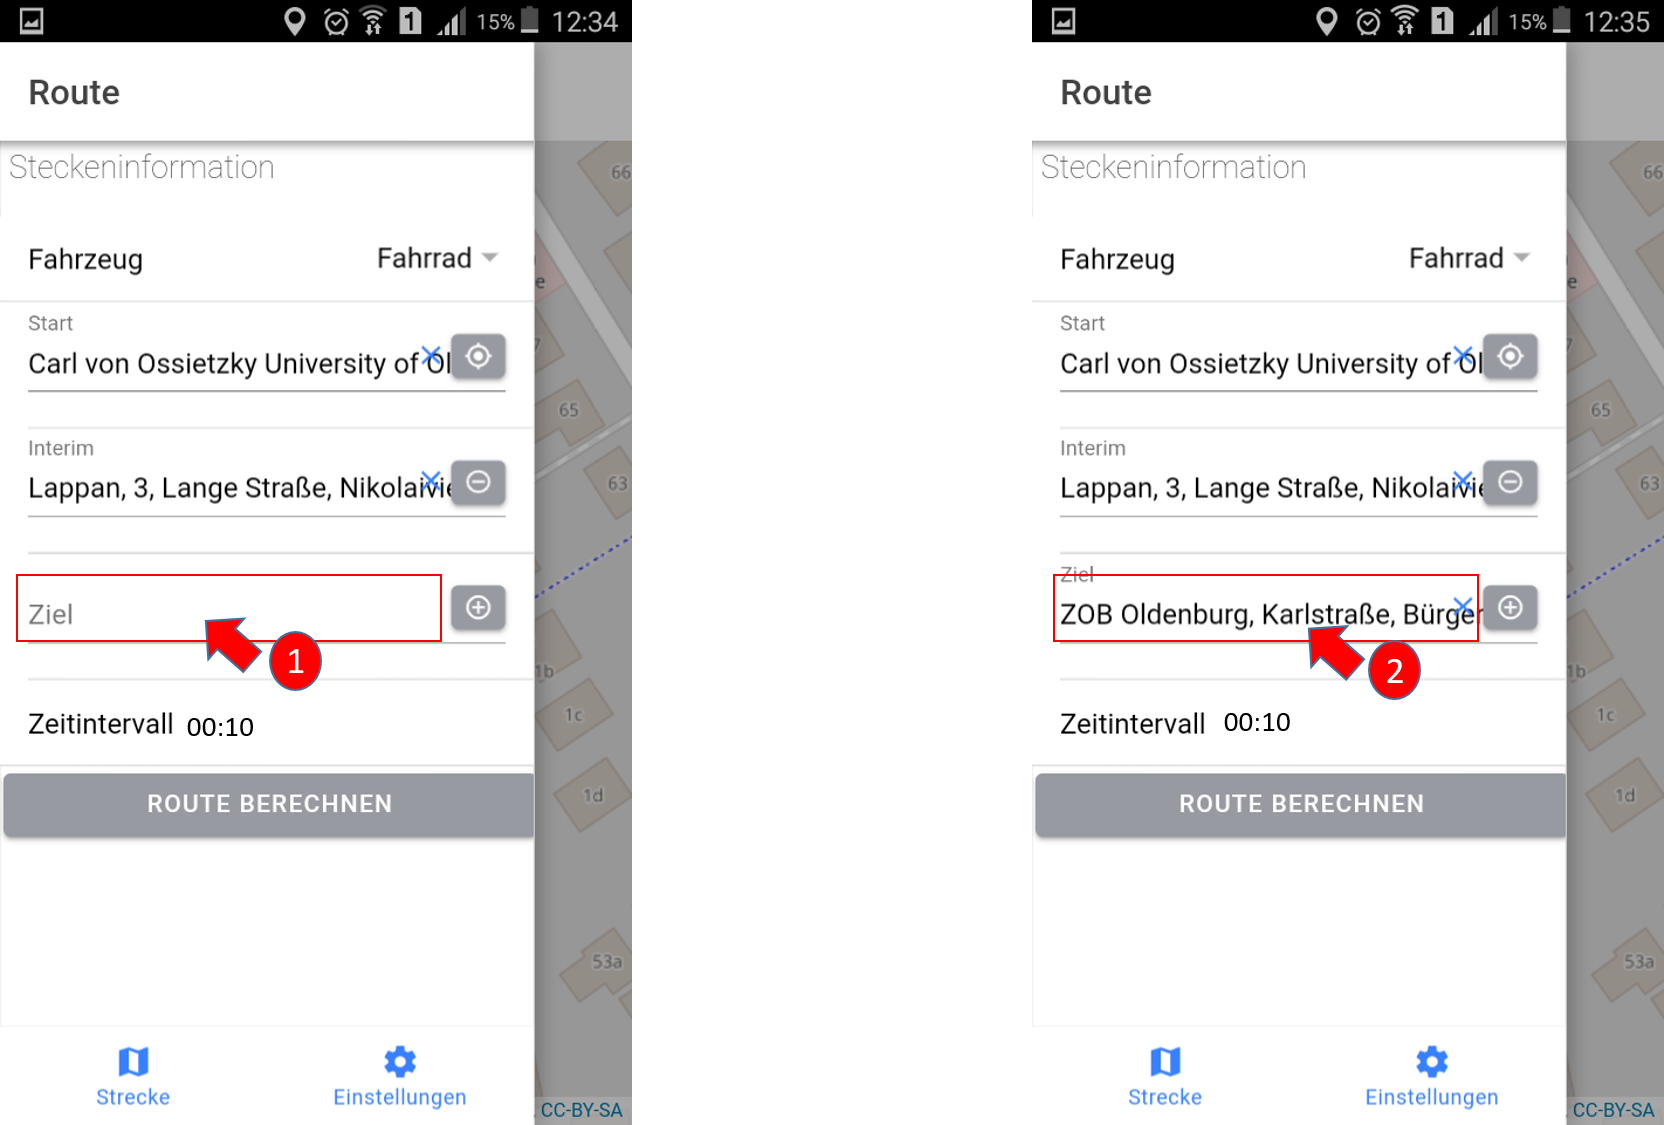
\includegraphics[height=8 cm]{./ressourcen/nutzerhandbuch/ziel.png}}
\caption{Zielpunkt}
\label{fig:app:Zielpunkt}
\end{figure}
 
\newpage
\paragraph{Routeneinstellungen:}
\begin{itemize}
  \item Tippen Sie auf die Schaltfläche Einstellungen, um die Routing-Einstellungen zu öffnen.\\
  Wie gezeigt in \Fig{app:Routeneinstellungen}.
  \item Wählen Sie Ihre Einstellungen für Umgebungsparameter. Diese Parameter haben Einfluss auf die Routenberechnung.
  	\begin{itemize}
  		\item Wählen Sie die maximalen PM10-Feinstaub- und Relevanzwerte.
  		\item Wählen Sie die maximalen PM25-Feinstaub- und Relevanzwerte.
  		\item Wählen Sie die minimalen und maximalen Temperaturwerte und die Relevanz der Temperatur.
	\end{itemize}
  \item Tippen Sie auf die Schaltfläche Strecke, um zur  Streckeninformation zurückzukehren
\end{itemize}

\begin{figure}[h!]
\centerline{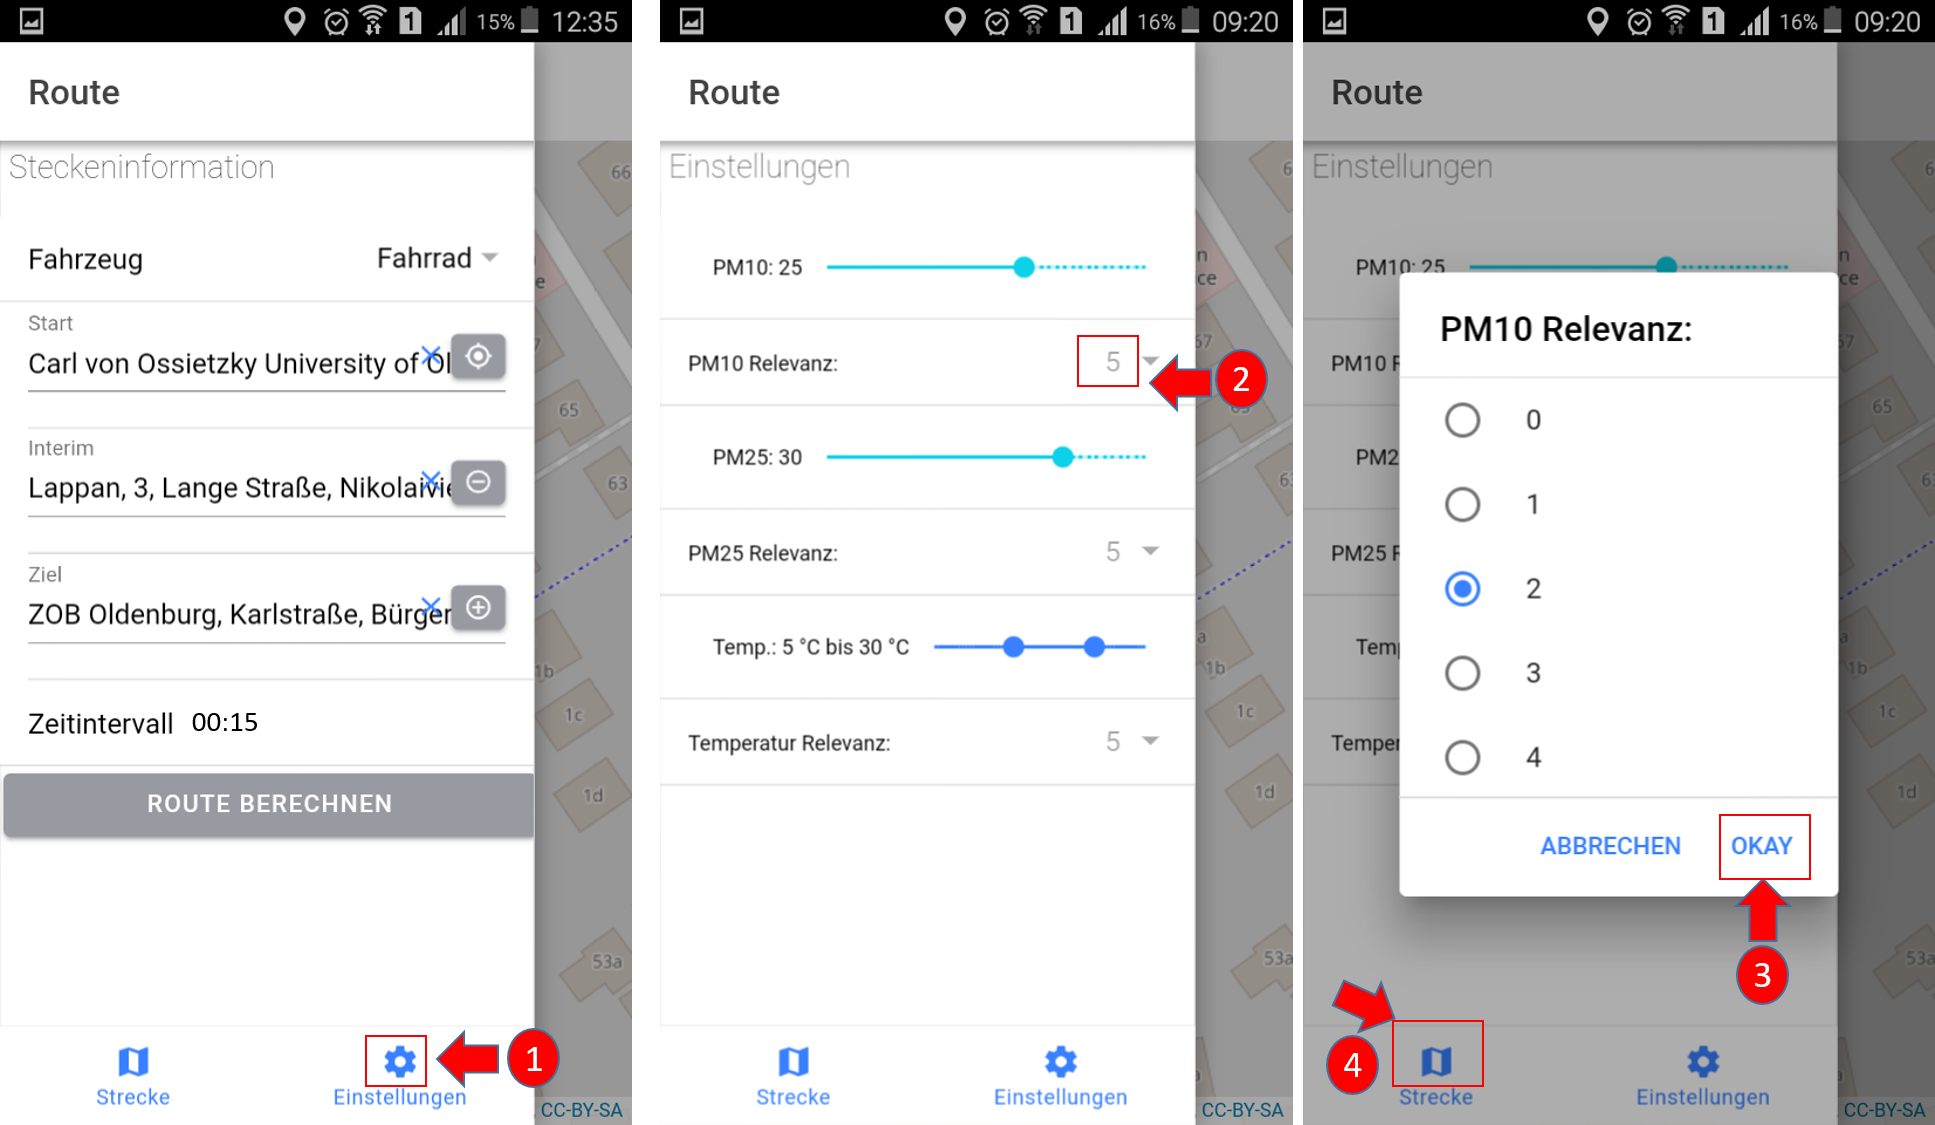
\includegraphics[height=8 cm]{./ressourcen/nutzerhandbuch/einstellungen.png}}
\caption{Routeneinstellungen}
\label{fig:app:Routeneinstellungen}
\end{figure} 

\newpage
\paragraph{Dynamisches Routing-Zeitintervall:}
In diesem Zeitintervall wird überprüft, ob es während der Navigation eine neue bessere Route gibt.\\
Wie gezeigt in \Fig{app:Dynamisches_Routing_Zeitintervall}.
\begin{figure}[h!]
\centerline{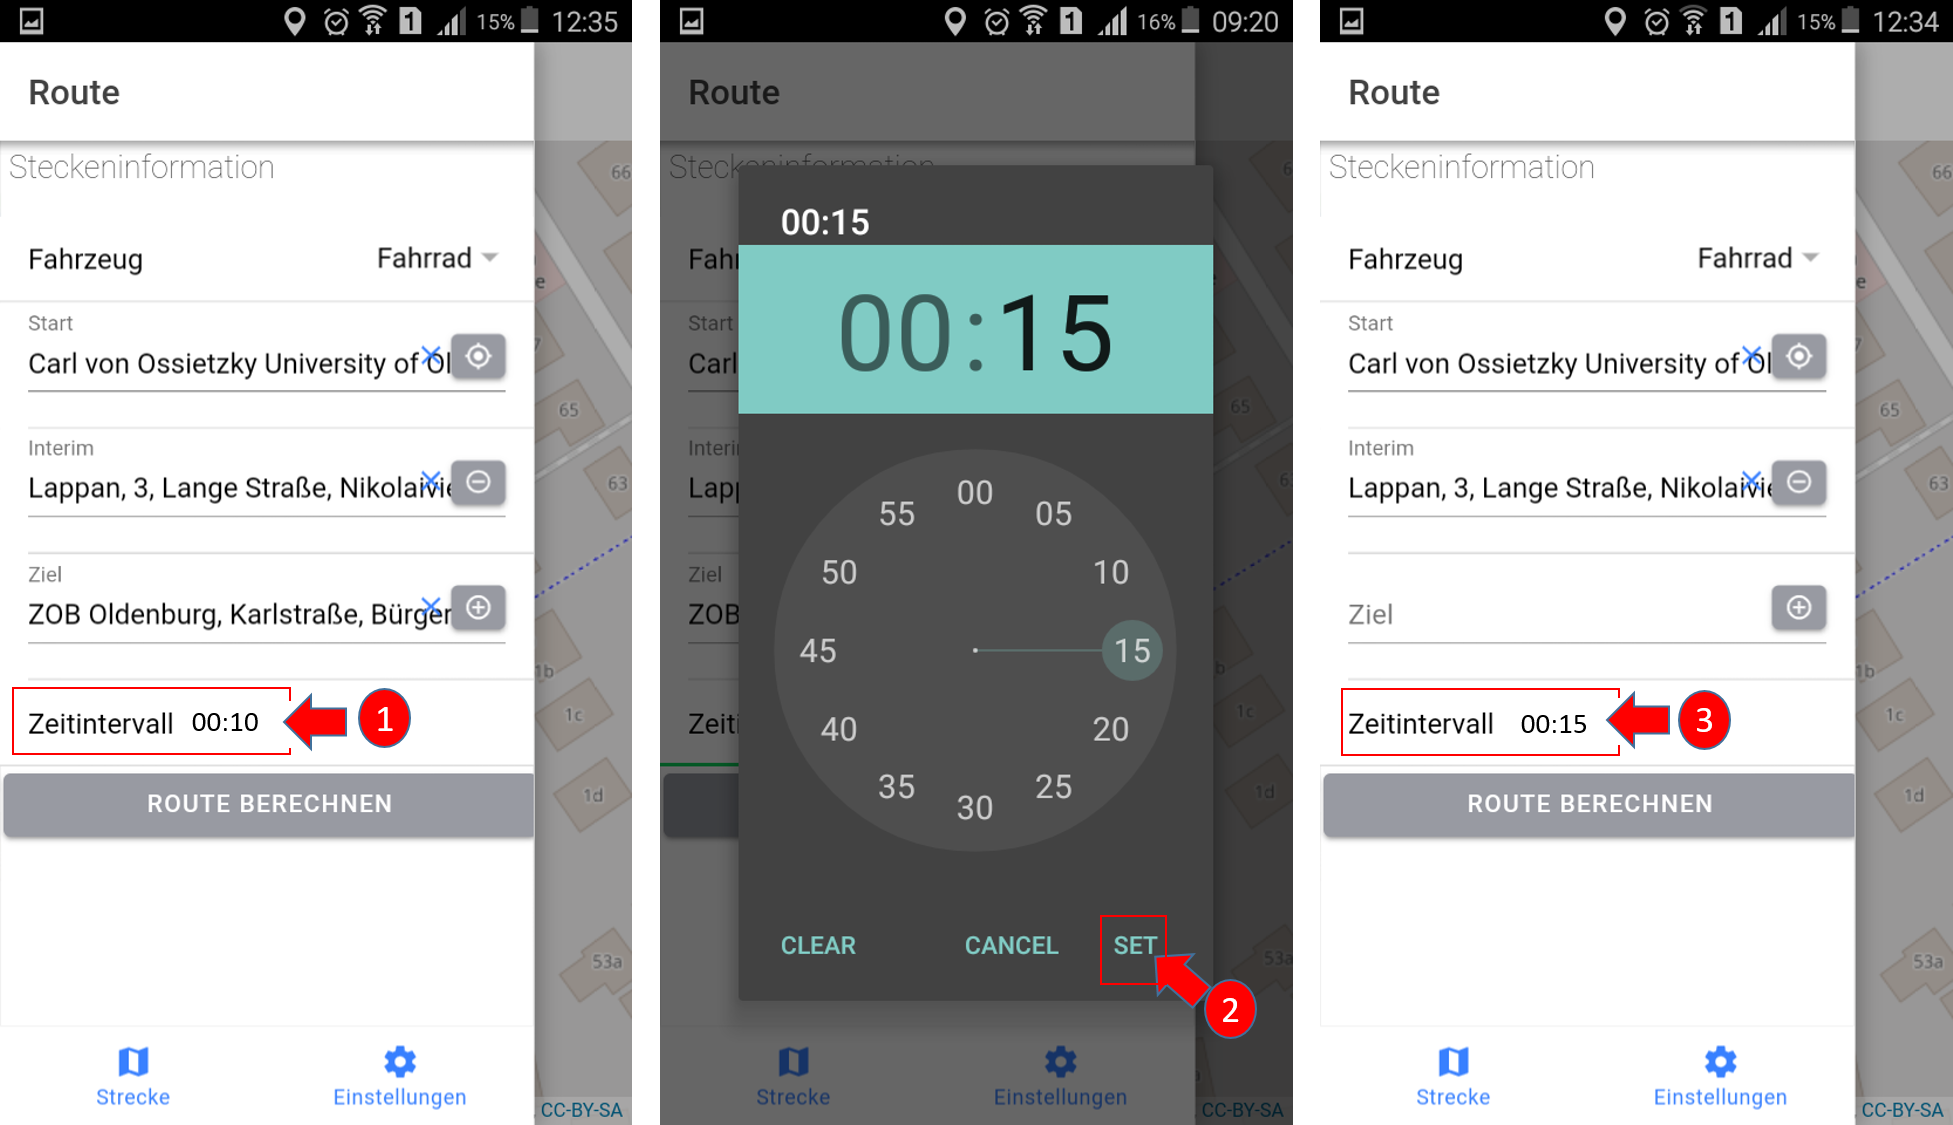
\includegraphics[height=6 cm]{./ressourcen/nutzerhandbuch/zeitintervall.png}}
\caption{Dynamisches Routing-Zeitintervall}
\label{fig:app:Dynamisches_Routing_Zeitintervall}
\end{figure} 

\paragraph{Fahrzeug:}
Wählen Sie Ihr Fahrzeug wie gezeigt in \Fig{app:Fahrzeug}.
\begin{figure}[h!]
\centerline{\includegraphics[height=6 cm]{./ressourcen/nutzerhandbuch/Fahrzeug.png}}
\caption{Fahrzeug}
\label{fig:app:Fahrzeug}
\end{figure} 


\paragraph{Route berechnen und Routen anzeigen:}
Nachdem Sie die Navigationspunkte ausgewählt haben, tippen Sie auf Route Berechnen, um eine Route zu berechnen.\\
Wie gezeigt in \Fig{app:route_berechnen_zwischen}.
\begin{itemize}
  \item Wenn die Navigationspunkte Zwischenziele enthalten, befindet sich nur eine Route zwischen dem Start und dem Ziel.
  
\begin{figure}[h!]
\centerline{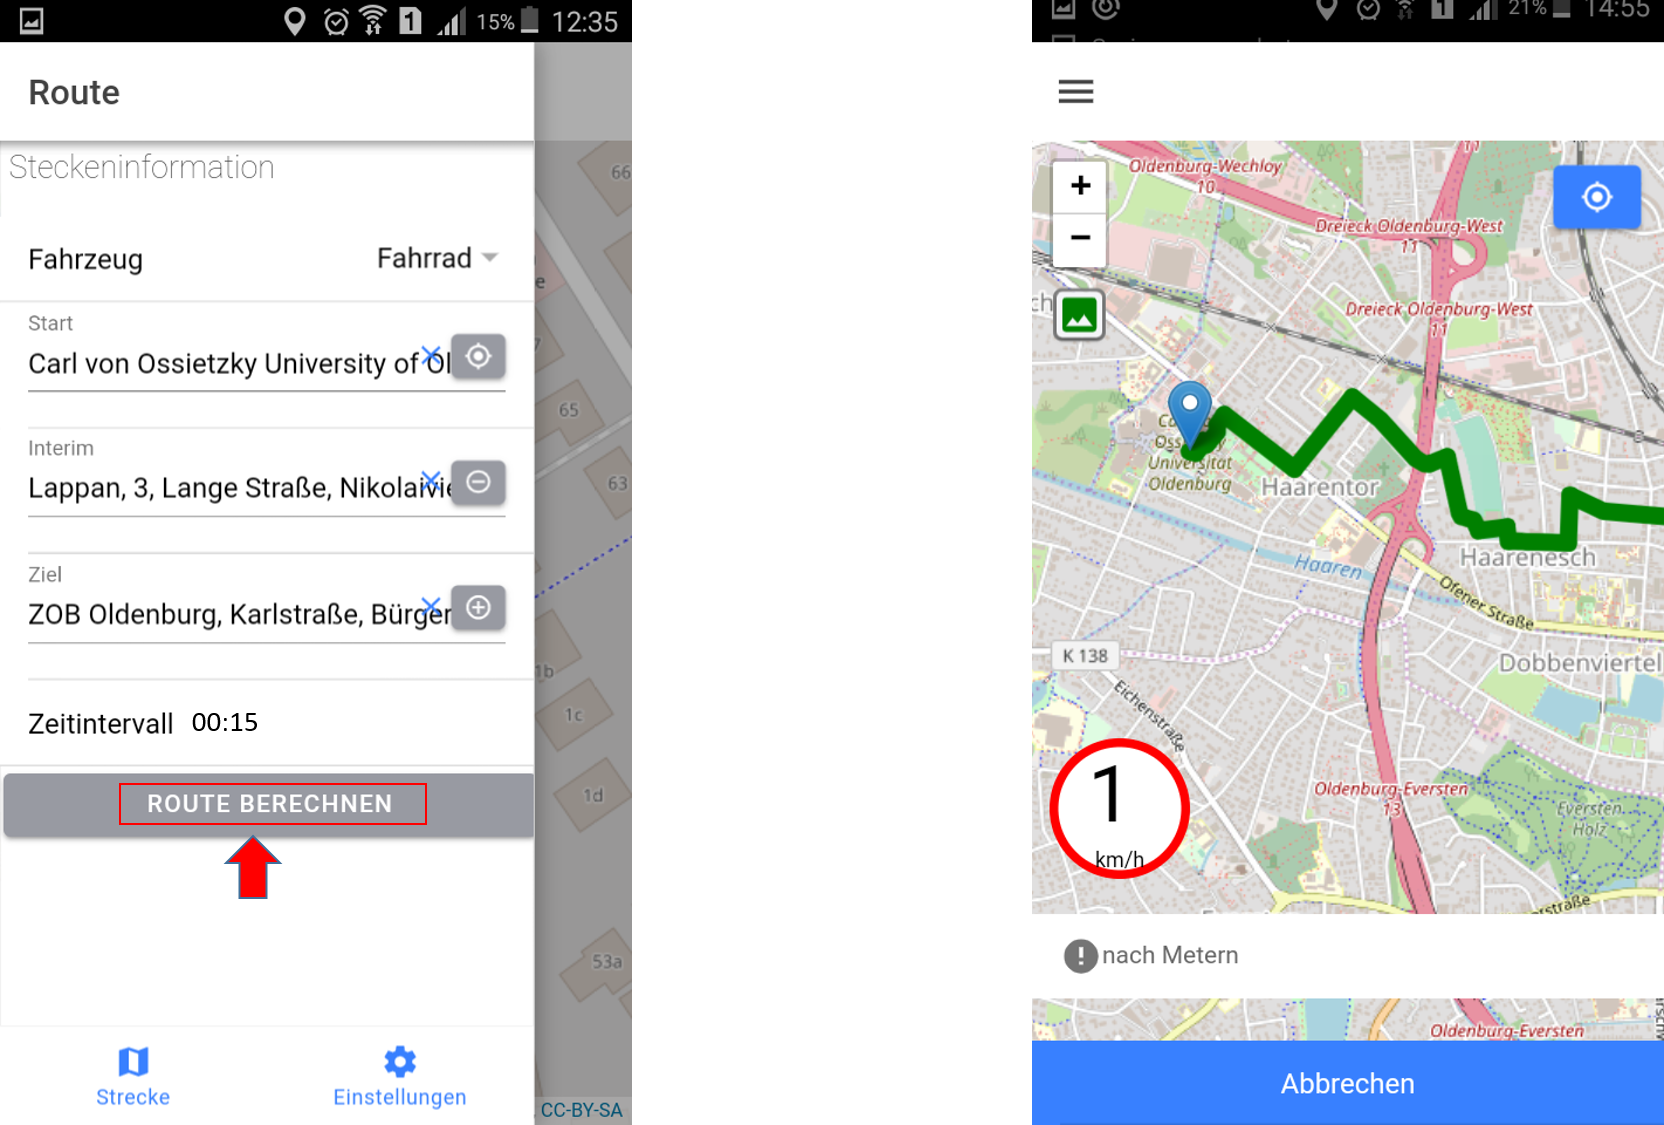
\includegraphics[height=8 cm]{./ressourcen/nutzerhandbuch/route_berechnen_zwischen.png}}
\caption{Route berechnen mit Zwischenziele}
\label{fig:app:route_berechnen_zwischen}
\end{figure} 

  \item Wenn die Navigationspunkte nur Start- und Zielpunkt enthälten, gibt es höchstens drei mögliche Routen.\\
  Wie gezeigt in \Fig{app:route_berechnen}.
  	\begin{itemize}
  		\item Um einen Route auszuwählen, tippen Sie auf die gewünschte Route.

  		\item Die beste Route ist grün, die zweitbeste blau und die drittbeste rot. Die gewählte Route ist visuell hervorgehoben.
	\end{itemize}
	
\begin{figure}[h!]
\centerline{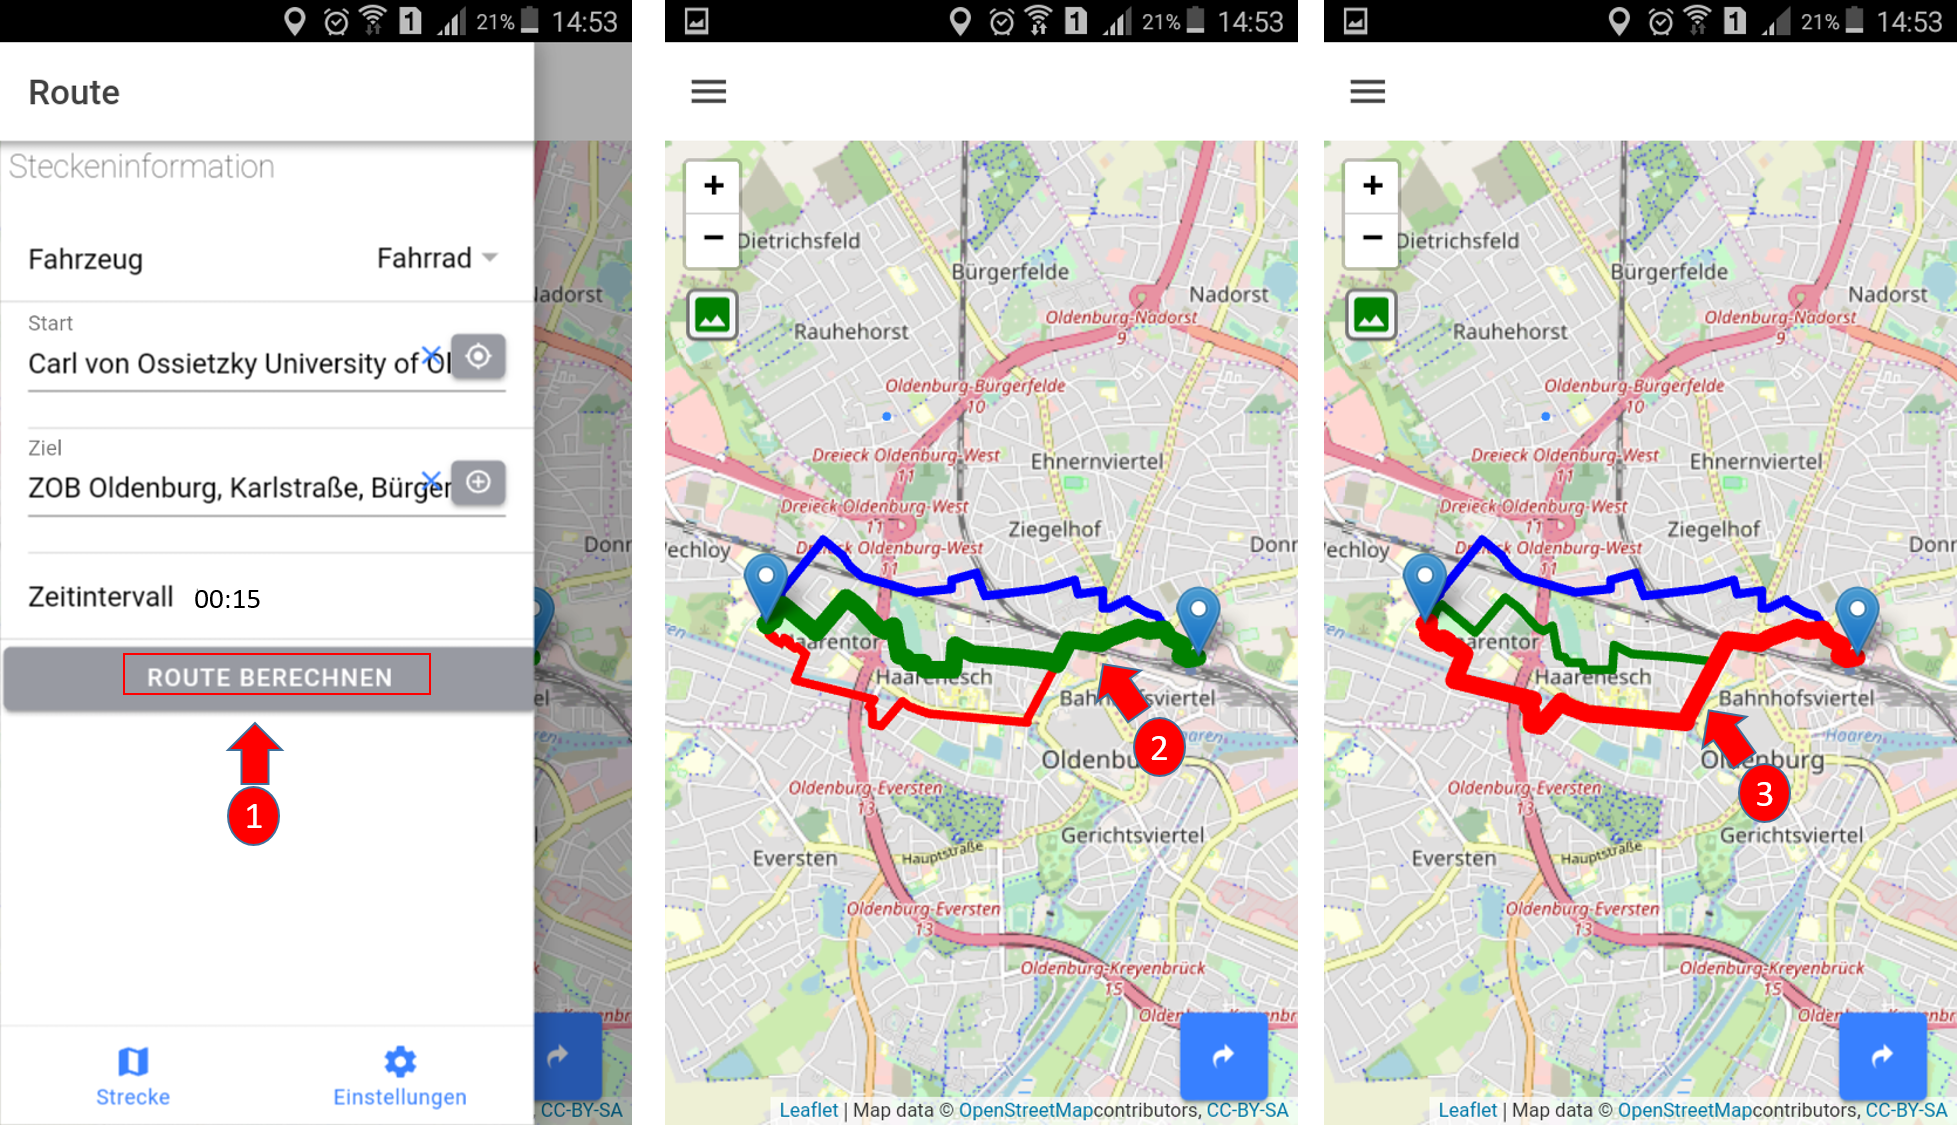
\includegraphics[height=8 cm]{./ressourcen/nutzerhandbuch/route_berechnen.png}}
\caption{Route berechnen ohne Zwischenziele}
\label{fig:app:route_berechnen}
\end{figure} 

\end{itemize}


\newpage
\paragraph{Navigieren:}
siehe \Fig{app:Navigieren}.
\begin{enumerate}
  \item Um die Navigation zu starten, tippen Sie auf die Navigationstaste. 
  \item Während der Navigation wird die aktuelle Position als blauer Kreis um die aktuelle Position angezeigt.
  \item Die Bewegungsgeschwindigkeit wird in einem roten Kreis links unten angezeigt.
  \item Die Navigationsanweisung wird unten angezeigt.
  \item Um die Navigation zu beenden, klicken Sie auf die Abbrechentaste.
  \item Wenn Sie auf die Navigationsanweisung klicken, wird eine Liste aller Navigationsanweisungen angezeigt.
\end{enumerate}

\begin{figure}[h!]
\centerline{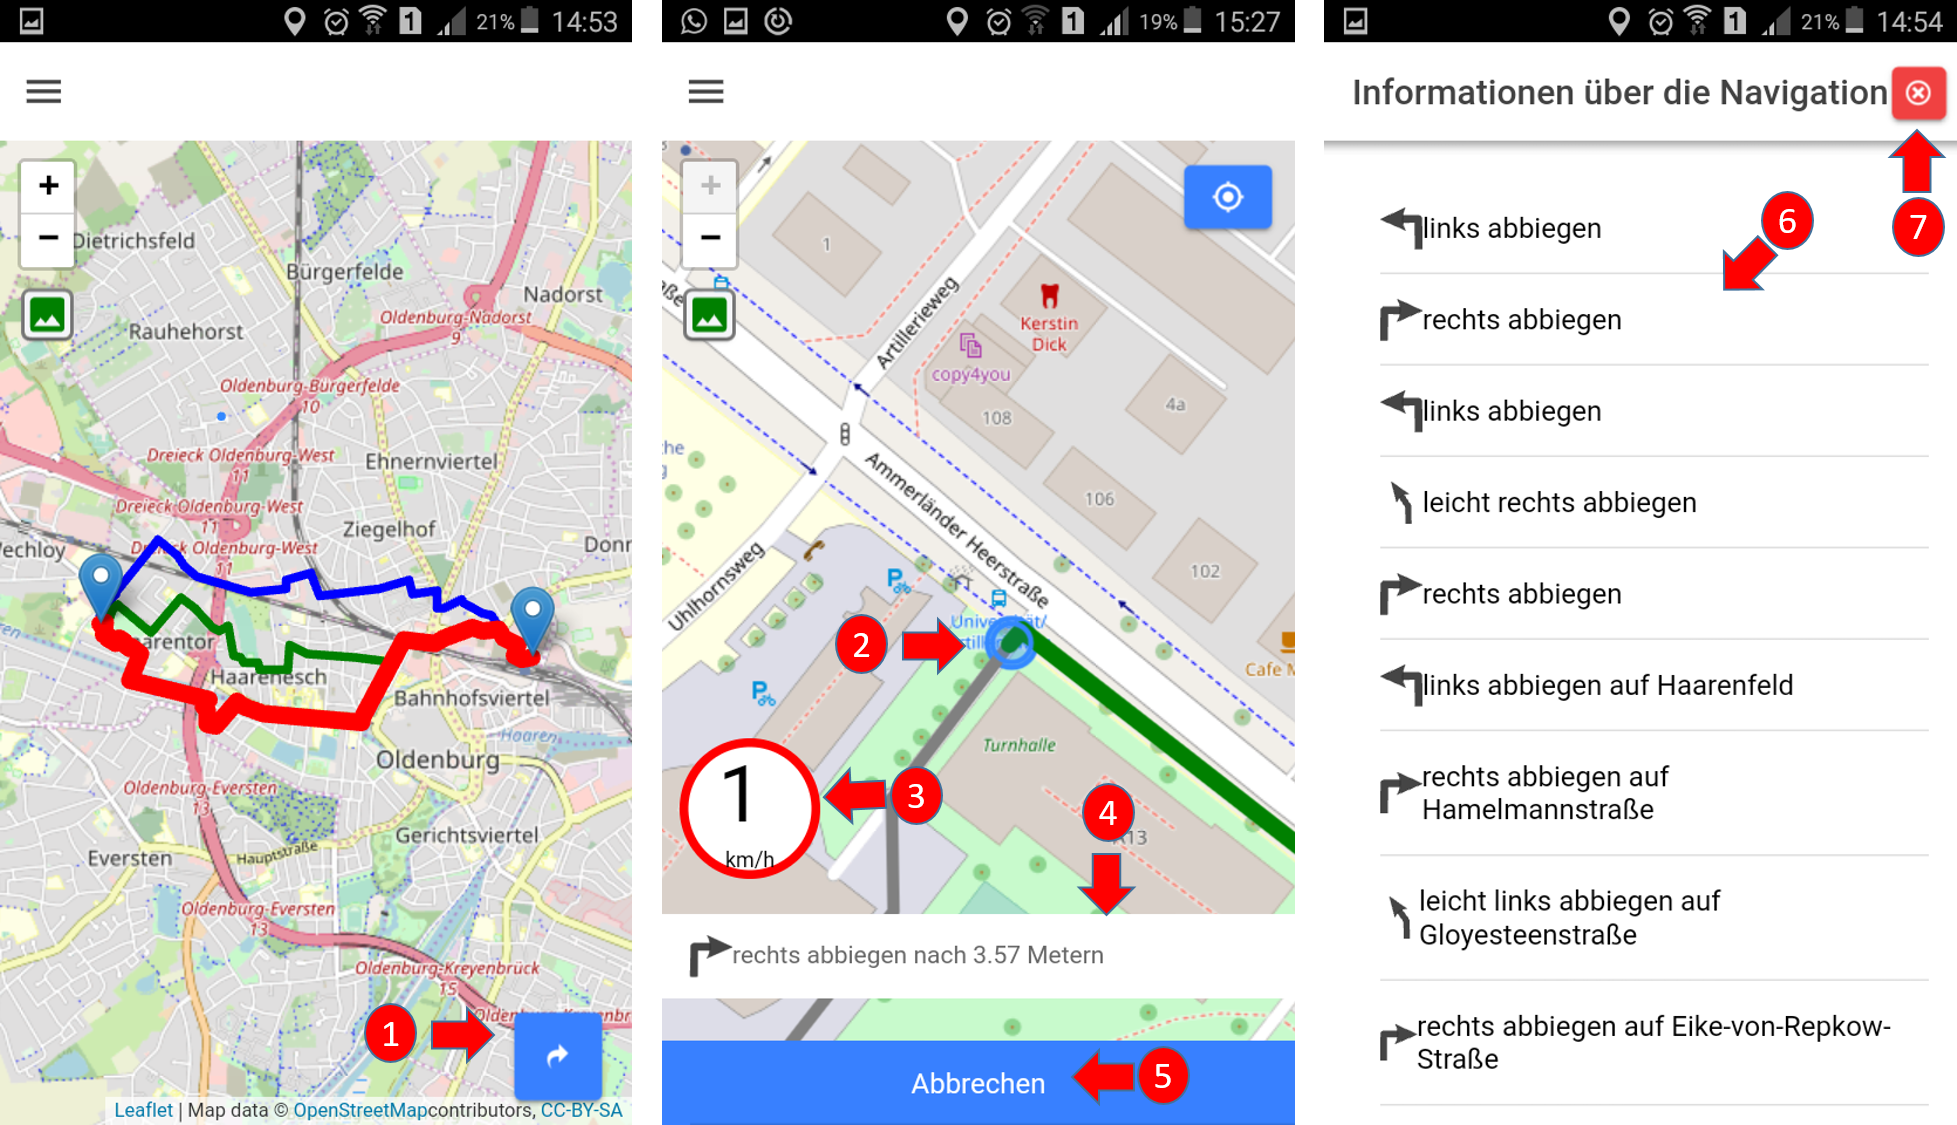
\includegraphics[height=8 cm]{./ressourcen/nutzerhandbuch/navigate.png}}
\caption{Navigieren}
\label{fig:app:Navigieren}
\end{figure}

\newpage
\paragraph{Heatmap:}
Um die Heatmap anzuzeigen, klicken Sie auf die Heatmap-Icon. Wie gezeigt in \Fig{app:heatmap}.\\
Die Heatmap zeigt, wie sich die Umgebungsparameter auf die Routenberechnung auswirken
\begin{figure}[h!]
\centerline{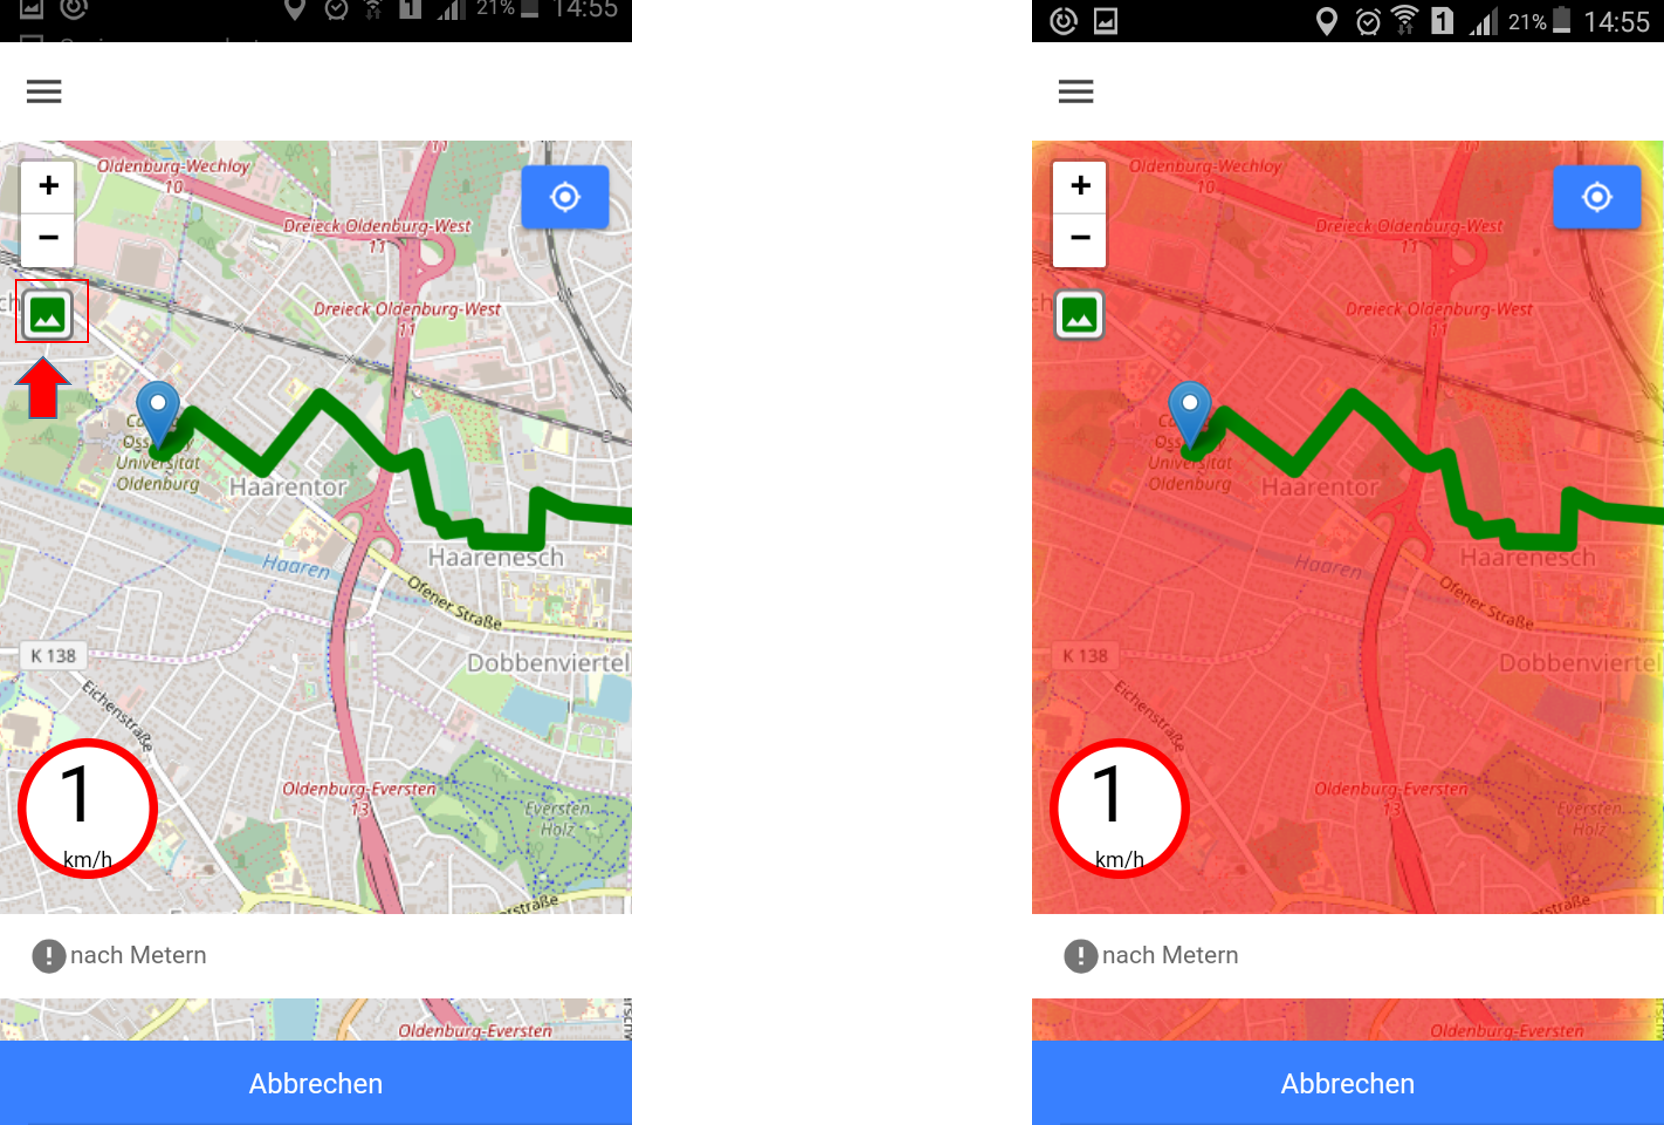
\includegraphics[height=6 cm]{./ressourcen/nutzerhandbuch/heatmap.png}}
\caption{heatmap}
\label{fig:app:heatmap}
\end{figure}



% Platzhalter für finale Einrückung
\let\levelone\section
\let\leveltwo\subsection
\let\levelthree\subsubsection

\levelone{Nutzerhandbuch \sk}
\label{sec:nutzerhandbuch:sk}
In den nachfolgenden Abschnitten wird die Inbetriebnahme und anschließende Konfiguration eines \sk erläutert.

\leveltwo{Überblick über die verwendete Hardware}
Für den Betrieb des Sensorknotens wird ein Mikrocontroller sowie angeschlossene Sensoren verwendet.
Als Mikrocontroller kommt eine NodeMCU ESP8266 zum Einsatz.
Im Standardaufbau werden zudem ein Nova SDS011 zur Messung von Feinstaub und ein BME280 zur Messung von Temperatur, Luftfeuchte und -druck verwendet.

\levelthree{NodeMCU ESP8266}
Diese Komponente ist das Herzstück der Sensorstation und besitzt neben der CPU ein WLAN Modul.
Dieses Board wird über einen MicroUSB"=Anschluss mit Strom versorgt.
Neben dem MicroUSB"=Anschluss gibt es 30 Pins, um Sensoren und/oder Aktuatoren anzuschließen.

\levelthree{SDS011}
Der Feinstaubsensor "Nova SDS011", der in den Sensorknoten eingebaut ist, misst Feinstaub der Partikelgröße PM 2,5 und PM 10.
Dabei wird das Prinzip der Laserstreuung ausgenutzt, indem die Partikel gemessen werden, die durch den gemessenen Bereich fliegen.
Die Laserstrahlen werden dann in elektrische Signale umgewandelt, die dann bereitgestellt werden können.
Dabei wird die Luft mit einem kleinen Lüfter durch den Bereich befördert.

\levelthree{BME280}
Der BME280 ist ein Sensor zur Messung der Temperatur, Luftfeuchtigkeit und Luftdruck.
Er eignet sich zum Anschluss an verschiedene Boards wie Arduino"=Boards oder den Raspberry Pi.
Der Sensor ist ideal zum Betrieb einer Wetterstation.

\leveltwo{Aufbau von einem \sk}
Die benötigten Komponenten, um einen \sk aufbauen zu können, sind in \Fig{skcomponents} abgebildet.

\begin{figure}[htb]
	\begin{minipage}{0.6\textwidth}
		\centering
		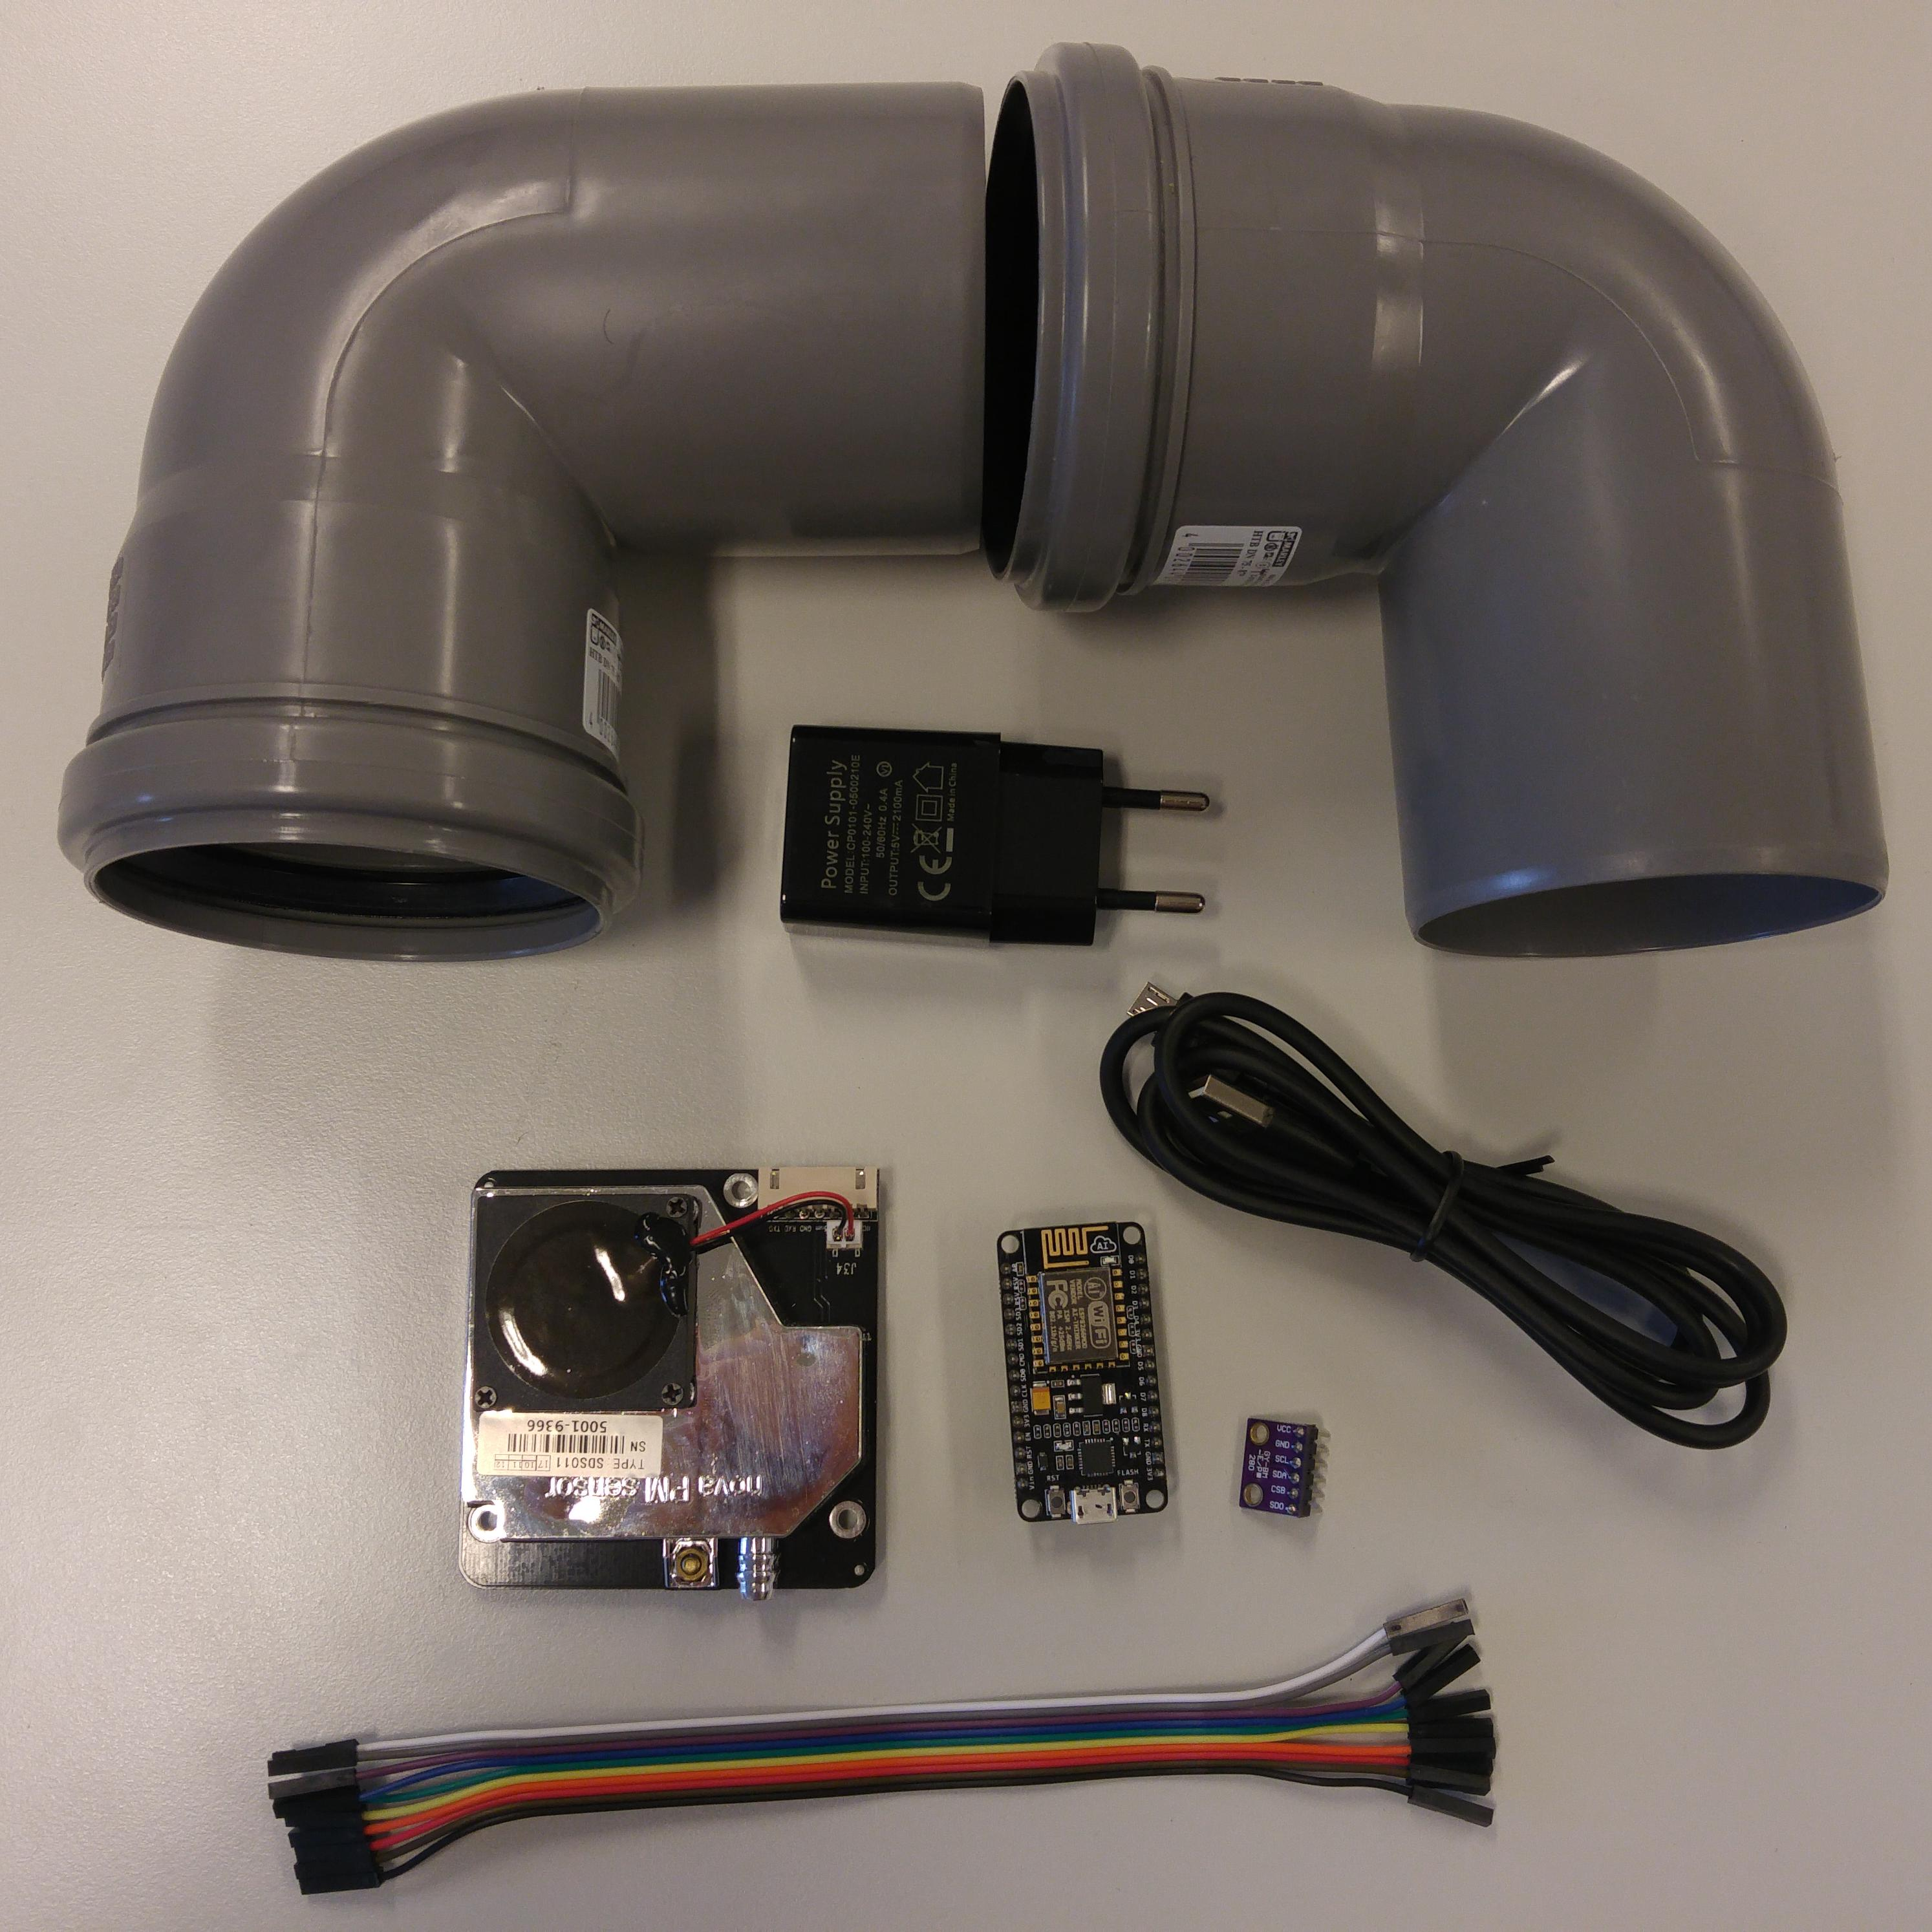
\includegraphics[width=\textwidth]{./ressourcen/SK-HardwareUeberblick.jpg}
	\end{minipage}
	\begin{minipage}{0.35\textwidth}
		\begin{itemize}
			\item 2x \SI{90}{^\circ} HT"=Bögen
			\item \SI{5}{V}"=Netzteil
			\item Micro"=USB"=Kabel
			\item SDS011
			\item NodeMCU
			\item BME280
			\item Jumper"=Kabel
			\item Schlauch mit \SI{6}{mm} Innendurchmesser
			\item \textbf{Optional:} 
			\begin{itemize}
				\item Kabelbinder zur Montage
			\end{itemize}
		\end{itemize}
	\end{minipage}
	\caption{Die benötigten Komponenten für einen \sk}
	\label{fig:skcomponents}
\end{figure}

Der Standardaufbau eines Sensorknotens kann aus \Fig{skwiringdefault} entnommen werden:

\begin{figure}[htb]
	\centering
	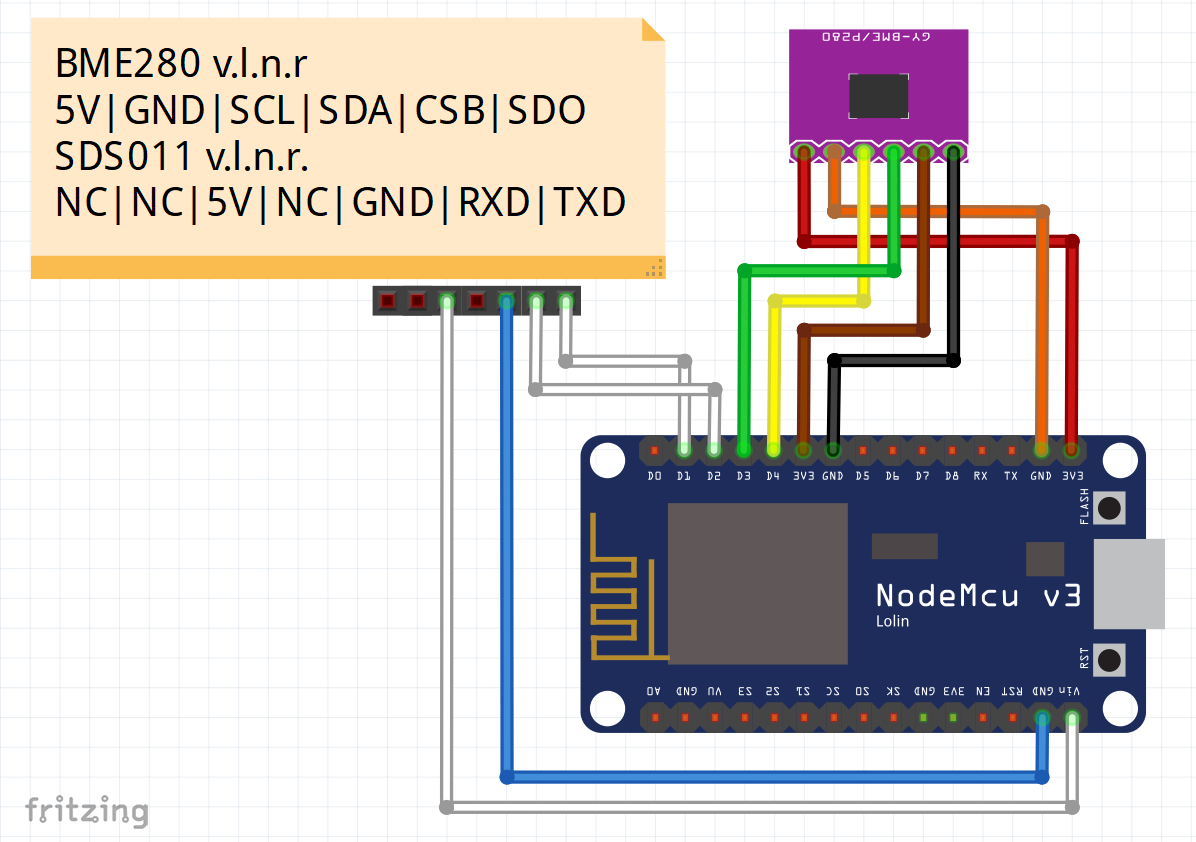
\includegraphics[width=0.8\textwidth]{./ressourcen/Prod_Verdrahtungsplan}
	\caption{Der Standard"=Verdrahtungsplan für den \sk}
	\label{fig:skwiringdefault}
\end{figure}

Beim Aufbau ist auf die korrekte Belegung der Pins zu achten. Obiges Bild gilt als Anschlussplan für die Standardkonfiguration.
Sollen andere Pins der NodeMCU verwendet werden, so muss dies der Software über eine angepasste Konfiguration mitgeteilt werden.

Nach dem Verkabeln der Komponenten können diese in die HT"=Bögen gesteckt werden.
Dabei ist auf die korrekte Ausrichtung des SDS011 zu achten, da dieser mit dem Lüfter nach unten montiert werden muss, wie in \Fig{skpositionsds011} gezeigt ist.

\begin{figure}[!htb]
	\centering
	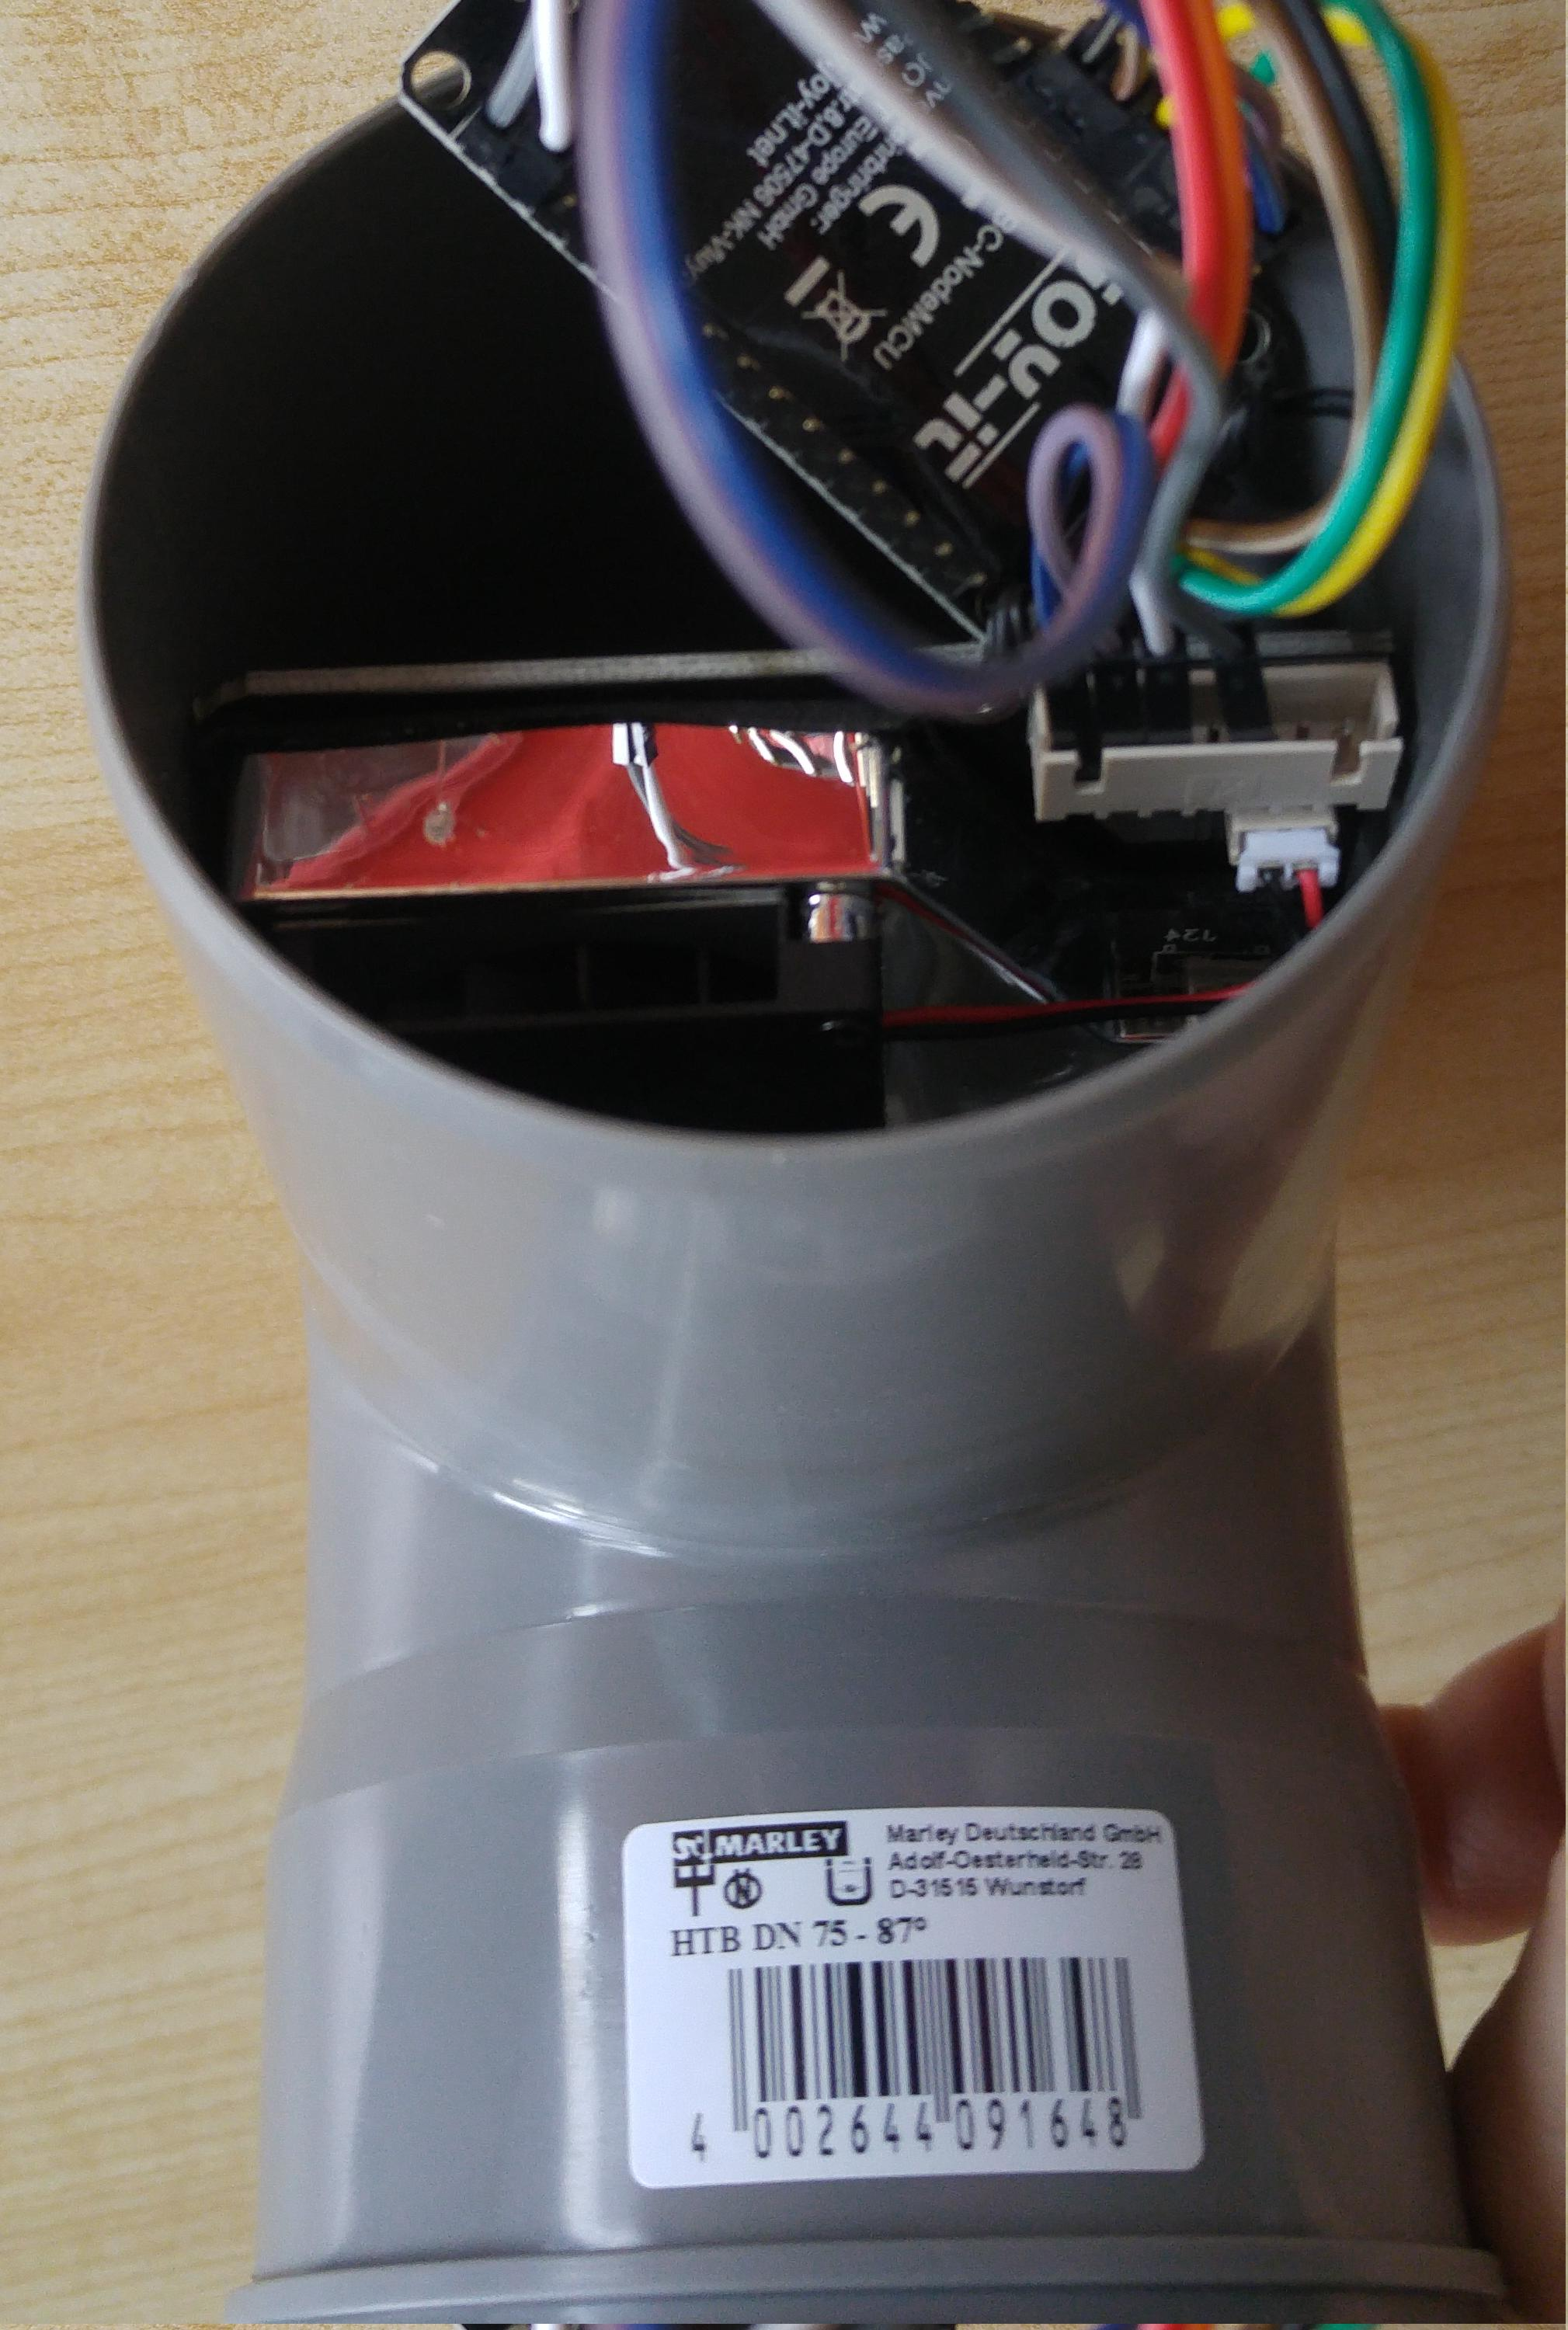
\includegraphics[width=0.6\textwidth]{./ressourcen/SK_AusrichtungSDS.jpg}
	\caption{Position des SDS011 innerhalb der HT"=Bögen}
	\label{fig:skpositionsds011}
\end{figure}


\leveltwo{Aufspielen der Firmware}
Nach dem Aufbau eines \sk geschieht das Aufspielen der Firmware über ein eigens in der \pg entwickeltes Installationstool (nur für Microsoft Windows).
Dieses kann über folgenden Link bezogen werden: \url{https://pg-rio-uis.informatik.uni-oldenburg.de/mitmachen}\footnote{\url{https://pg-rio-uis.informatik.uni-oldenburg.de/assets/tools/PGRIO-SK-Config-Tool.exe}}
\FloatBarrier

Nach dem Starten des Installationstools erscheint das Registrierungs- bzw. Anmeldeformular, abgebildet in \Fig{skitool01}.
\begin{figure}[!htb]
	\centering
	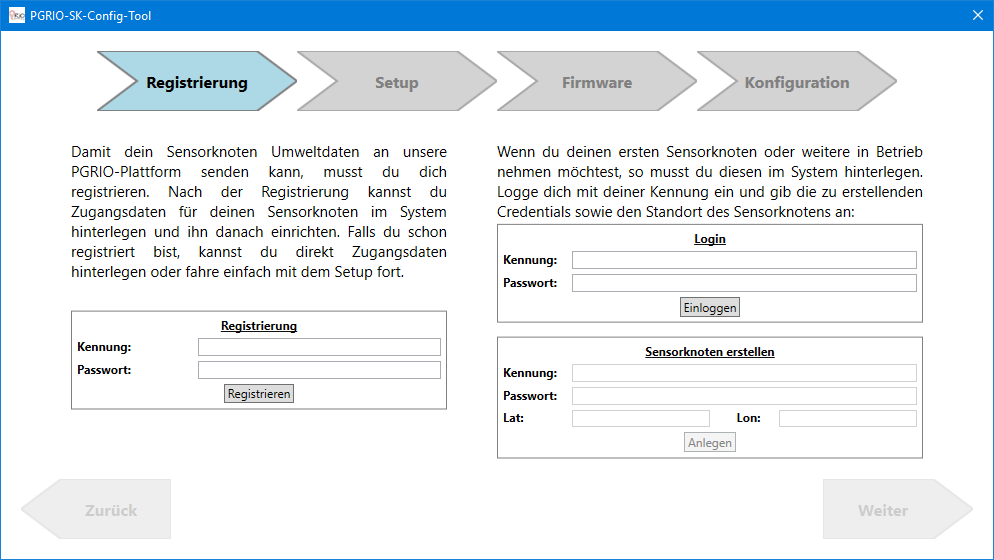
\includegraphics[width=0.8\textwidth]{./ressourcen/i-tool/Registrierung}
	\caption{Die Startseite des Installationstool}
	\label{fig:skitool01}
\end{figure}
Hier kann ein neuer Benutzer (Kennung und Passwort) angelegt werden, der den Eigentümer des \sk repräsentiert.
Mit dieser Nutzerkennung kann dann nach dem Einloggen ein neuer \sk angelegt werden.
Dabei ist zu beachten, dass die Kennung des Sensorknotens mit dem Präfix \textit{pgrio-} beginnen muss.

\begin{mdframed}[frametitle=Weitere Hinweise]
	\begin{minipage}{\linewidth}
	    \begin{itemize}
	        \item Es ist darauf zu achten, dass in der Kennung, sowie dem Passwort keine Sonderzeichen verwendet werden dürfen.
	        \item Fehleingaben werden vom Installationstool abgefangen und durch eine Meldung im unteren Bereich angezeigt.
	        \item Bei länger andauernden Operationen wird ein Ladebildschirm eingeblendet.
	        \item Bei Problemen mit dem Installationstool sollte frühzeitig ein Ansprechpartner der \pg kontaktiert werden.
	    \end{itemize}
	\end{minipage}
\end{mdframed}

Ist der \sk erfolgreich angelegt, erfolgt mit einem Klick auf \PicDet{Weiter} das Setup der Seriellen Verbindung.
Dies ist in \Fig{skitool02} abgebildet.
\begin{figure}[!htb]
    \centering
    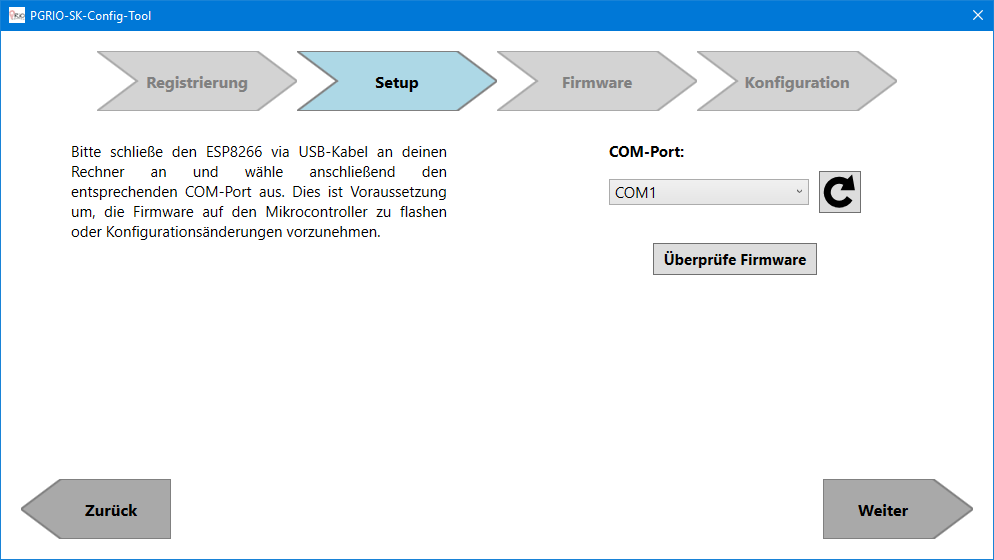
\includegraphics[width=0.8\textwidth]{./ressourcen/i-tool/Setup}
    \caption{Auswahl des Com"=Ports im Installationstool}
    \label{fig:skitool02}
\end{figure}
Hier kann der \PicDet{Com"=Port} ausgewählt werden, mit dem die Verbindung zum \sk aufgebaut werden soll.
Mit dem Button \PicDet{Überprüfe Firmware} kann darüber hinaus überprüft werden, ob bereits eine Firmware im Rahmen dieser \pg auf den \sk aufgespielt worden ist.

\begin{mdframed}[frametitle=Hinweis]
	\begin{minipage}{\linewidth}
    	Falls die Verbindung mit dem \sk über keinen \PicDet{Com"=Port} erfolgreich ist, oder kein \PicDet{Com"=Port} zur Auswahl steht, sollten die verwendeten Treiber für die NodeMCU überprüft werden.
	\end{minipage}
\end{mdframed}

Ist die Verbindung zum \sk erfolgreich hergestellt, kann über einen Klick auf den \PicDet{Weiter}"=Button die Firmware"=Seite aufgerufen werden.
Diese ist in \Fig{skitool03} abgebildet.
\begin{figure}[!htb]
	\centering
	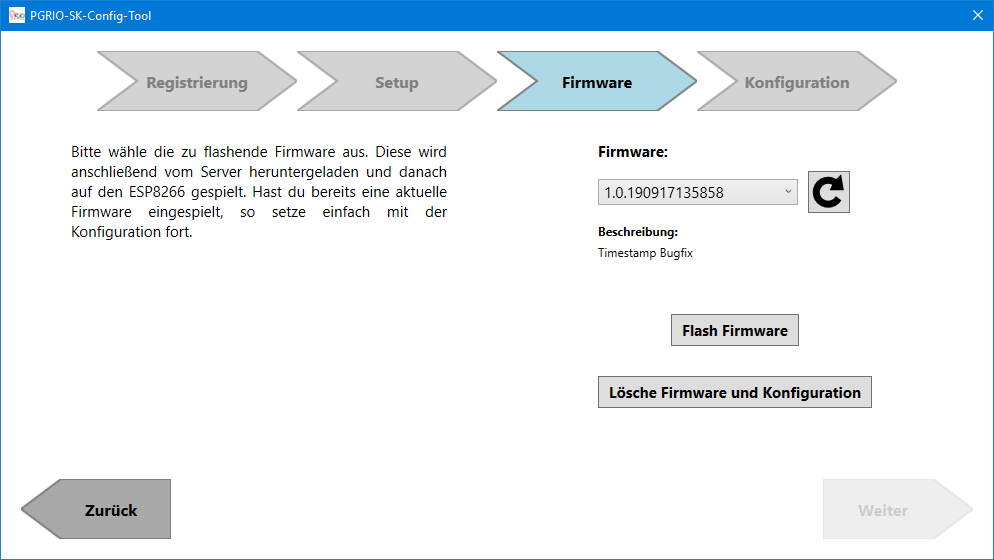
\includegraphics[width=0.8\textwidth]{./ressourcen/i-tool/Firmware}
	\caption{Flashen der \skfw im Installationstool}
	\label{fig:skitool03}
\end{figure}
Hier kann über einen Klick auf den Button \PicDet{Flash Firmware} die Firmware auf den \sk aufgespielt werden.
Zu Testzwecken kann darüber hinaus auch eine spezifische Firmware"=Version über die Auswahl"=Box aufgespielt werden.

\begin{mdframed}[frametitle=Hinweis]
	\begin{minipage}{\linewidth}
    	Sollte bei der späteren Konfiguration etwas fehlschlagen, sodass der \sk nicht mehr über das Installationstool konfiguriert werden kann, kann der gesamte \sk über den Button \PicDet{Lösche Firmware und Konfiguration} in den Werkszustand zurückgesetzt werden.
   \end{minipage}
\end{mdframed}

Sobald die Firmware auf den \sk aufgespielt ist, muss die NodeMCU über den Reset-Knopf neugestartet oder kurzzeitig vom PC getrennt und neu verbunden werden. Nach ca. fünf Sekunden kann über einen Klick auf den \PicDet{Weiter}"=Button die Konfigurations"=Seite aufgerufen werden.
Diese ist in \Fig{skitool05} abgebildet.
\begin{figure}[!htb]
	\centering
	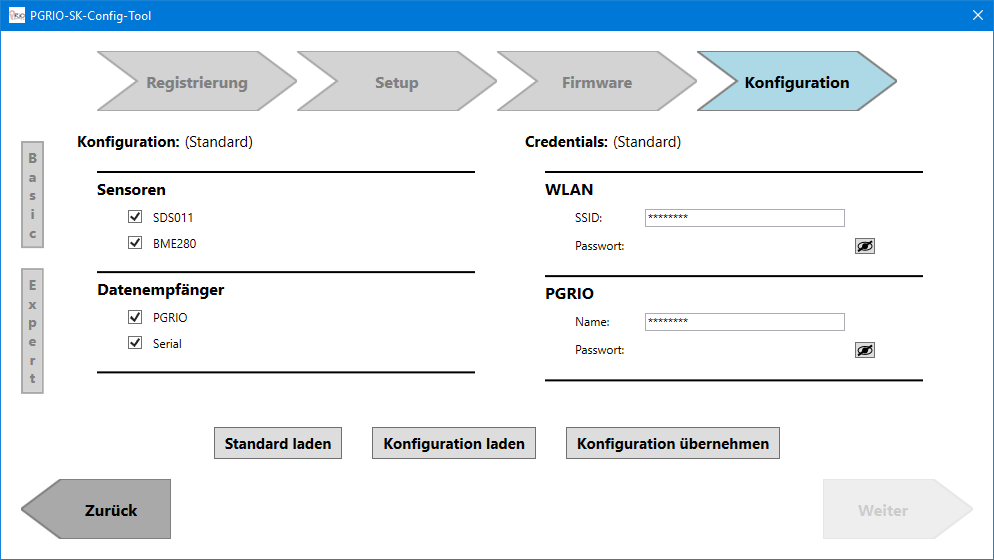
\includegraphics[width=0.8\textwidth]{./ressourcen/i-tool/Konfiguration_basic}
	\caption{Die einfache Konfiguration im Installationstool}
	\label{fig:skitool05}
\end{figure}
Hier kann die angeschlossene Hardware konfiguriert werden, sowie die Zugangsdaten zum WLAN und der IoT"=Plattform (Kennung von der Registrierungs"=Seite) eingegeben werden.
Über einen Klick auf den Button \PicDet{Konfiguration übernehmen} werden diese auf den \sk gespeichert.

\begin{mdframed}[frametitle=Weitere Hinweise]
	\begin{minipage}{\linewidth}
	    \begin{itemize}
	        \item Über den Button \PicDet{Standard laden} kann die Standardkonfiguration wiederhergestellt werden. Diese wird jedoch erst über einen Klick auf den Button \PicDet{Konfiguration übernehmen} gespeichert.
	        \item Über den Button \PicDet{Konfiguration laden} kann eine bereits gespeicherte Konfiguration vom \sk geladen werden.
	        \item Über einen Klick auf den Button \PicDet{Expert} kann in den Expertenmodus gewechselt werden. Dieser wird in \Fref{sec:skitoolExpert} beschrieben.
	    \end{itemize}
	\end{minipage}
\end{mdframed}

\leveltwo{Erweiterte Konfiguration}
\label{sec:skitoolExpert}
Im Experten"=Modus des Installationstools (siehe \Fig{skitool06}) kann die Konfiguration als \filename{.json}"=Datei editiert werden.

\begin{figure}[htb]
	\centering
	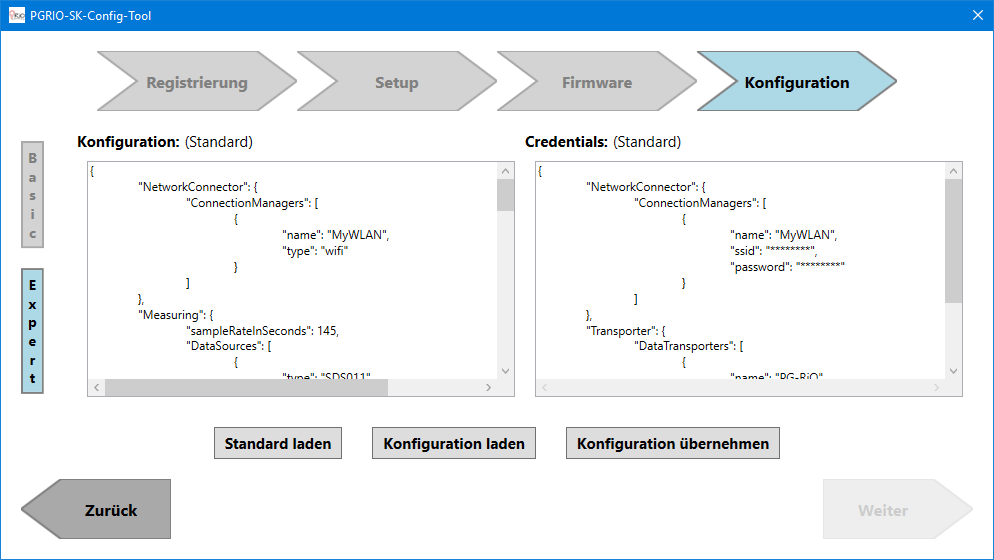
\includegraphics[width=0.8\textwidth]{./ressourcen/i-tool/Konfiguration_expert}
	\caption{Die erweiterte Konfiguration im Installationstool}
	\label{fig:skitool06}
\end{figure}

Dabei können weitergehende Einstellungen vorgenommen werden, die über die einfache Inbetriebnahme eines \sk hinausgehen.

Die Standardkonfiguration sieht dabei wie folgt aus:

\begin{lstlisting}[language=json,basicstyle=\footnotesize]
{
  "NetworkConnector": {
    "ConnectionManagers": [
      {
        "name": "MyWLAN",
        "type": "wifi"
      }
    ]
  },
  "Measuring": {
    "sampleRateInSeconds": 145,
    "DataSources": [
      {
        "type": "SDS011",
        "sdsTxPin": "D1",
        "sdsRxPin": "D2"
      },
      {
        "type": "BME280",
        "bmeSdaPin": "D3",
        "bmeSclPin": "D4"
      }
    ]
  },
  "MeasurementSender": {
    "DataSinks": [
      {
        "type": "PG-RiO",
        "transporterName": "PG-RiO",
        "transformerWhitelist": [
          "ALL"
        ]
      },
      {
        "type": "SerialDump",
        "transformerWhitelist": [
          "ALL"
        ]
      }
    ]
  },
  "Transporter": {
    "DataTransporters": [
      {
        "type": "MQTT_TLS",
        "hostOrIp": "pg-rio-iot.informatik.uni-oldenburg.de",
        "port": 8883,
        "publicKey": "pg-rio-iot",
        "name": "PG-RiO"
      },
      {
        "type": "HTTPS",
        "hostOrIp": "pg-rio-sensors-update.informatik.uni-oldenburg.de",
        "port": 443,
        "publicKey": "pg-rio-sensors-update",
        "name": "PG-RiO-Update"
      }
    ]
  },
  "TimeManager": {
    "TimeSyncStrategies": [
      {
        "type": "NTP",
        "serverName": "pool.ntp.org"
      }
    ]
  },
  "Updater": {
    "cyclic": {
      "transporterName": "PG-RiO-Update",
      "intervalInHours": 24
    }
  },
  "StatusInformation": {
    "sendIntervalInSeconds": 600,
    "transporterName": "PG-RiO"
  }
}
\end{lstlisting}

Die Standardcredentials sieht wie folgt aus:

\begin{lstlisting}[language=json,basicstyle=\footnotesize]
{
  "NetworkConnector": {
    "ConnectionManagers": [
      {
        "name": "MyWLAN",
        "ssid": "********",
        "password": "********"
      }
    ]
  },
  "Transporter": {
    "DataTransporters": [
      {
        "name": "PG-RiO",
        "user": "********",
        "password": "********"
      }
    ]
  }
}
\end{lstlisting}

In den weiteren Abschnitten werden die Einträge weiter erläutert.

\levelthree{NetworkConnector}
Im Bereich NetworkConnector werden verschiedene Verbindungsoptionen für die NodeMCU angegeben, damit er eine Internet"=Verbindung verfügbar hat und gemessene Werte an die IoT"=Plattform senden kann.
In diesem Falle wird ein \textit{ConnectionManager} vom Typ \textit{wifi} mit Namen \textit{MyWLAN} angegeben.
Die Credentials dazu werden mit der selben Struktur in der \filename{credentials.json} passend hinterlegt.
Das Mapping erfolgt dabei über das Attribut \textit{name}.
Diese müssen entsprechend des verfügbaren WLANs angepasst werden.

\levelthree{Measuring}
Im Measuring wird das Messverfahren konfiguriert.
Es werden das Messintervall, sowie die angeschlossenen Sensoren (\textit{DataSources}) konfiguriert.
Aktuell werden die Sensoren \textit{SDS011} und der \textit{BME280} unterstützt.
Für den SDS011 muss angegeben werden, mit welchen Pins der NodeMCU sein TX- sowie RX"=Pin verbunden sind und für den BME280 die zugehörigen Pins seines SDA- sowie SCL"=Pins.
Darüberhinaus können Offsets für die Messwerte angegeben werden.
Wird bei einer Kalibrierung festgestellt, dass der gemessene Wert für beispielsweise PM2.5 systematisch um \SI{5}{\micro g/m^3} vom tatsächlichen Wert abweicht, so kann dies entsprechend konfiguriert werden.
Dabei werden die Offsets für die PM"=Werte über die Schlüssel \textit{offsetPM2.5} bzw. \textit{offsetPM10} in \SI{0,1}{\micro g/m^3} angegeben und die des BME280 über die Schlüssel \textit{offsetTemperature} in \SI{0,01}{^{\circ}C}, \textit{offsetPressure} in \SI{0,01}{hPa} sowie \textit{offsetHumidity} in \SI{0,01}{\%}.

\levelthree{MeasurementSender}
Hier werden die Ziele (\textit{DataSinks}) für die gemessenen Umweltdaten definiert.
Oben wird eine DataSink vom Typ \textit{PG"=RiO} konfiguriert, mit der Messdaten im PG"=RiO"=Format aufbereitet werden, damit sie von der IoT"=Plattform verstanden werden.
Zudem wird der verwendete DataTransporter zum Versenden der Daten über seinen Namen angegeben.

\begin{mdframed}[frametitle=Hinweis]
	\begin{minipage}{\linewidth}
		Die Typen der DataSink und des DataTransporters müssen kompatibel sein, siehe \Fref{sec:userhb:compdsdt}.
	\end{minipage}
\end{mdframed}

Darüberhinaus wird eine Liste der verwendeten DataSources dieser DataSink angegeben.
Das Schlüsselwort \textit{ALL} bedeutet, dass alle verfügbaren Sensoren verwendet werden.

\levelthree{Transporter}
Unter Transporter werden mehrere \textit{DataTransporters} angegeben.
Diese sind für den Datenverkehr verantwortlich.
Z.B. muss ein DataTransporter angegeben werden, mit dem die gemessenen Umweltwerte versendet werden können.
Im Standardfall wird ein \textit{MQTT}"=DataTransporter konfiguriert, der mit dem Host \url{pg-rio-iot.informatik.uni-oldenburg.de} verbunden wird.
Dazu muss in der \filename{credentials.json} ein gültiger User und ein Passwort angegeben werden, um sich am Server zu authentifizeiren.
Das Mapping erfolgt dabei wieder über das Attribut \textit{name}.
\begin{mdframed}[frametitle=Hinweis]
	\begin{minipage}{\linewidth}
		\begin{itemize}
			\item Für den \text{MQTT}"=DataTransporter auf dem Host \url{pg-rio-iot.informatik.uni-oldenburg.de} muss der Public"=Key vom Server mit dem in der Firmware hinterlegten Key übereinstimmen.
			\item Der Port ist in dieser Konstellation fix auf 8884 festgelegt.
		\end{itemize}
	\end{minipage}
\end{mdframed}

\levelthree{TimeManager}
Aus Umweltdaten werden Umweltinformationen, wenn sie u.a. einen Zeit- und Raumbezug haben.
Damit die gemessenen Werte also dem tatsächlichen Zeitpunkt der Messung zugeordnet werden können, muss der Mikrocontroller seine Systemzeit synchronisieren.
Dazu werden \textit{TimeSyncStrategies} verwendet.
Im obigen Fall wird eine \textit{NTP}"=Strategie angegeben, mit deren Hilfe die Systemzeit mit dem angegebenen NTP"=Server (hier \url{pool.ntp.org}) synchronisiert wird.

\levelthree{Updater}
Hier wird das automatische Update konfiguriert.
Aktuell kann ausschließlich eine zyklische Überprüfung angegeben werden.
Dort wird das Prüf"=Intervall in Stunden und der zugehörige DataTransporter angegeben, über den auf Updates geprüft wird. Mittels selben DataTransporter werden vorhandene Updates auch heruntergeladen.
\begin{mdframed}[frametitle=Hinweis]
	\begin{minipage}{\linewidth}
		\begin{itemize}
			\item Für den \text{HTTPS}"=DataTransporter auf dem Host \url{pg-rio-iot.informatik.uni-oldenburg.de} muss der Public"=Key vom Server mit dem in der Firmware hinterlegten Key übereinstimmen.
			\item Der Port ist in dieser Konstellation fix auf 444 festgelegt.
		\end{itemize}
	\end{minipage}
\end{mdframed}

\levelthree{StatusInformation}
Hier wird festgelegt, wie häufig der Sensorknoten Statusinformationen melden soll.
Dazu werden das Sendeintervall in Sekunden angegeben und der DataTransporter angegeben, über der die Informationen gesendet werden.
Statusinformationen beinhalten z.B. die Laufzeit seit dem letzten Neustart.

\levelthree{Kompatibilität von DataSink mit DataTransporter}
\label{sec:userhb:compdsdt}
Da nicht jede \textit{DataSink} mit jedem \textit{DataTransporter} kompatibel ist, sind die möglichen Kombinationen in \Tbl{skconfcomp} abgebildet.

\begin{table}[htb]
	\centering
	\caption{Kompatibilität von DataSink mit DataTransporter}
	\begin{tabular}{|l|l|}
		\hline
		Typ der DataSink & kompatible DataTransporters \\ \hline
		PG"=RiO & MQTT, Serial \\ \hline
		SerialDump & Serial \\ \hline
	\end{tabular}
\label{tbl:skconfcomp}
\end{table}

\begin{mdframed}[frametitle=Hinweis]
	\begin{minipage}{\linewidth}
		Der Serial"=DataTransporter wird über die leere Zeichenkette "" identifiziert und muss in der Konfiguration unter DataTransporters nicht aufgeführt werden.
	\end{minipage}
\end{mdframed}

\section{Bekannte Bugs und Einschränkungen}
\label{sec:bugsundeinschraenkungen}
In diesem Abschnitt werden alle bekannten Bugs und Einschränkungen des PG RiO Systems aufgelistet. Die Auflistung der Bugs und Einschränkungen erfolgt nach dem Schema, wie Bug Tickets in Jira gepfelgt werden. Im Folgenden folgt eine Auflistung aller Bugs und Einschränkungen:

\begin{enumerate}
	\item \textbf{Was habe ich gemacht, um den Fehler zu erzeugen?} \newline
	Ich habe versucht mich an der IoT-Plattform mit gültigen Zugangsdaten zu authentifizieren. \newline
	\textbf{Was ist das erwartete Verhalten?}\newline
	Ich habe erwartet ein Token zu bekommen \newline
	\textbf{Was ist das beobachtete Verhalten?} \newline
	Die IoT-Plattform antwortet mit einem 500 er Fehler \newline
	\textbf{Lösung} \newline
	Sobald die Verbindung zur Datenbank abbricht können sich die Services nicht mehr mit der Datenbank verbinden. Somit kann kein externer Dienst mehr authentifiziert werden sowie auch keine Daten mehr abfragen
	\item \textbf{Was habe ich gemacht, um den Fehler zu erzeugen?} \newline
	Ich habe versucht in der Development Umgebung einen neuen MQTT Client mit Zugangsdaten zu dem Password File hinzuzufügen \newline
	\textbf{Was ist das erwartete Verhalten?}\newline
	Der MQTT Client kann sich danach mit den Zugangsdaten an dem MQTT-Broker anmelden \newline
	\textbf{Was ist das beobachtete Verhalten?} \newline
	Die Zugangsdaten haben keine Auswirkung, weil der MQTT-Broker offen ist. Das bedeutet, dass sich jeder Client ohne Authentifizierung an dem MQTT-Broker anmelden kann \newline
	\textbf{Lösung} \newline
	Da auf dem Development-System noch der Eclipse Mosquitto als MQTT-Broker läuft, sollte der neue MQTT-Broker, HiveMQ, eingerichtet werden. Somit würde die Authentifizierung, wie geplant, über den Identity-Service laufen und die Tools zum Anlegen von MQTT Client würden auch auf dem Development-System richtig funktionieren.
	\item \textbf{Was habe ich gemacht, um den Fehler zu erzeugen?} \newline
	Ich habe versucht Umweltdaten von dem Development-System zu exportieren. \newline
	\textbf{Was ist das erwartete Verhalten?}\newline
	Ich erhalte eine CSV Datei \newline
	\textbf{Was ist das beobachtete Verhalten?} \newline
	Ich bekomme keine CSV Datei \newline
	\textbf{Lösung} \newline
	Der Export wurde aus der Development Umgebung entfernt, weil dieser Probleme bezüglich der Datenbank verursacht hat. 
\end{enumerate} 
